%% March 21, 2002 version

%%  This file is called procdocs.tex
%
%%%%%%%%%%%%%%%%%%%%%%%%%%%%%%%%%%%%%%%%%%%
%%%%%%%%%
%%%%%
%% LaTeX Documentation file for Articles in
%% Proceedings Style Published by 
%% Kluwer Academic Press
%%
%%%%%%%%%%%%%%%%%%%%%%%%%%%%%%%%%%%%%%%%%%%
%%%%%%%%%
%%%%%
%% 
%%%%%%%%%%%%%%%%%%%%%%%%%%%%%%%%%%%%%%%%%%%
%%%%%%%%%
%%%%%
%% Macros written by
%% Amy Hendrickson
%% TeXnology, Inc.
%% 57 Longwood Avenue
%% Brookline, Massachusetts  02446
%% 617 / 738-8029
%%
%% Technical help: dthelp@wkap.com
%%
%%%%%%%%%%%%%%%%%%%%%%%%%%%%%%%%%%%%%%%%%%%
%%%%%%%%%
%%%%%

\def\thisdoc{Kluwer Proceedings Documentation}
\def\currstyle{Proceedings}

%% LaTeX2e 
%% Uncomment documentclass, and, optionally, 
%%                            the \usepackage command:
 \documentclass{kapproc} % Computer Modern font calls
 \usepackage{procps}% PostScript font calls
\usepackage[dvipsone]{graphicx}

\let\savenewpage\newpage

\pagenumbering{arabic}
\newdimen\abovetitleskip
\abovetitleskip=24pt

\voffset-1in
\newif\ifdotoc
\dotoctrue

\makeatletter
\ifdotoc
{\def\numberline#1{}
\def\contentsline#1#2#3{}\@starttoc{toc}}\fi
\def\l@section{\@dottedtocline{1}{1.5em}{2.3em}}
\def\@dottedtocline#1#2#3#4#5{\ifnum #1>\c@tocdepth \else
\item #4 \qquad{\it #5}\fi}
\setcounter{tocdepth}{1}
\def\numberline#1{}

\def\l@section{\vfill\@dottedtocline{1}{1.5em}{2.3em}}
\makeatother

%% fake versions of commands to make them work in documentation:

\let\openright\relax

%% <== end fake versions
\newdimen\savetopskip
\savetopskip=\topskip
\topskip=36pt

\let\savechapter\chapter
\let\savesection\section
\let\savesubsection\subsection

\let\StartOnNewPage\relax

\textwidth=6in
\hsize=6in
\linewidth=6in

\newdimen\savehsize
\newdimen\savetextwidth
\savehsize=\textwidth
\savetextwidth=\textwidth

\textheight=9in
\newdimen\saveparindent
\newdimen\saveparskip
\saveparindent=\parindent
\saveparskip=\parskip
\parindent=0pt
\parskip=6pt

\makeatletter

\newif\ifdoctitle
\global\doctitletrue
\def\ps@headings{\def\@oddfoot{\hfill}%
\def\@evenfoot{\hfill}%
%
\def\@evenhead{\ifdoctitle\global\doctitlefalse\hfill\else
\hbox to0pt{\hbox to\savetextwidth{%
\hskip-24pt\Large\bf\thepage\hskip 24pt%
\sqbullet\hskip10pt\sqbullet\hskip10pt
\Large\bf Using the Kluwer Macros
\hskip10pt\sqbullet\hskip10pt\sqbullet\hskip10pt\sqbullet\hfill}% 
\hss}\hfill\fi}
%                                    % left heading.
\def\@oddhead{\hbox to0pt{\hbox to\savetextwidth{%
\hfill\hbox{}\ifdoctitle\global\doctitlefalse\hfill\else
\hfill\sqbullet\hskip10pt\sqbullet\hskip 10pt\sqbullet\hskip10pt
\Large\bf Proceedings Style\hskip10pt%
\sqbullet\hskip10pt\sqbullet\hskip24pt\thepage\fi\hbox to-24pt{}}\hss}\hss}
% right heading.
}

\ps@headings

\oddsidemargin 12pt \evensidemargin  -12pt

\leftmargini=18pt
\labelsep=6pt

\def\sqbullet{\raise.2ex\hbox{\vrule width 4pt height4pt}}

\let\savelabelitemi\labelitemi

\def\labelitemi{%\llap
{\hbox to6pt{\sqbullet\hfill}}}



\def\ysection#1{\ifdotoc
\addcontentsline{toc}{section}{\protect\numberline{x}#1}\fi
{\let\uppercase\relax
\@startsection {section}{3}{-24pt}{-36pt plus -1pt minus 
 -1pt}{1sp}{\Large\bf}*{#1}}}

\def\section{\ysection}

\def\ysubsection#1#2{{\let\uppercase\relax%
\@startsection {subsection}{2}{-12pt}{-24pt plus -1pt minus 
 -1pt}{1sp}{\large\sc}#1{#2}}}

\def\subsection{\ysubsection*}

\let\savesubsubsection\subsubsection
\def\subsubsection{\savesubsubsection*}

\def\chapter#1{\global\doctitletrue
\vbox to  9.5pc{
\hyphenpenalty=10000 % No hyphenation in chapter heads
\parindent=-36pt
\vskip12pt\vskip-\parskip
\def\\ {\vskip-\parskip}
\booktitlefont\baselineskip=30pt
#1
\vskip1sp %8pt
\moveright-36pt\vbox{\advance\hsize by 36pt
\hrule height 1.5pt  width \hsize
}\vfill}}

\let\save@listI\@listI
\let\save@listi\@listi

\def\code{\vskip3pt
\hbox to\textwidth{\vrule width \textwidth height .6pt}
\normalsize\vskip1sp}

\def\endcode{\vskip6pt}
\let\xcode\code

\def\results{\bgroup
\let\pagestyle\eatone
\let\thispagestyle\eatone
\let\newpage\relax
\hbox to\hsize{.\dotfill.}
\vskip15pt
\bgroup
\def\contentsline##1##2##3{}
\def\addcontentsline##1##2##3{}
\def\addtocontents##1##2{}
\let\@listI\save@listI
\let\@listi\save@listi \@listi
\linewidth=\savehsize
\hsize=\savehsize
\textwidth=\savetextwidth
\parindent=\saveparindent
\parskip=\saveparskip
\let\chapter\savechapter
\let\section\savesection
\let\subsection\savesubsection
\let\subsubsection\savesubsubsection
\let\labelitemi\savelabelitemi
\normalsize\par}


\def\endresults{\vskip1sp
\egroup\vskip1sp\egroup
\hbox to\textwidth{\vrule width \textwidth height .6pt}
\xmedium\vskip18pt}

\def\nolineendresults{\vskip1sp
\egroup\vskip1sp\egroup
\xmedium\vskip18pt}

\def\xresults{\bgroup
\bgroup
\topskip\savetopskip
\def\contentsline##1##2##3{}
\let\@listI\save@listI
\let\@listi\save@listi \@listi
\linewidth=\savehsize
\hsize=\savehsize
\textwidth=\savetextwidth
\parindent=\saveparindent
\parskip=\saveparskip
\let\section\savesection
\let\subsection\savesubsection
\let\labelitemi\savelabelitemi
\normalsize\par}


\def\xendresults{\vskip1sp
\egroup\vskip1sp\egroup
\xmedium\vskip18pt}


\def\spresults{\hbox to\savehsize{\dotfill}
\vskip3pt\bgroup
\let\@listI\save@listI
\let\@listi\save@listi \@listi
\linewidth=\savehsize
\hsize=\savehsize
\textwidth=\savetextwidth
\parindent=\saveparindent
\parskip=\saveparskip
\normalsize}


\def\endspresults{\vskip3pt\egroup
\hbox to\textwidth{\vrule width \textwidth height .6pt}
\vskip18pt\xmedium}


\def\@listI{\leftmargin\leftmargini \parsep 4\p@ plus2\p@ minus\p@
\topsep 4\p@ plus2\p@ minus4\p@
\itemsep -3pt %4\p@ plus2\p@ minus\p@
}

\let\@listi\@listI
\@listi

\def\xmedium{\@setsize\xmedium{12pt}\xipt\@xipt}

\makeatother

\def\btt#1{{\tt\string\ \unskip#1}}
\def\lc{$\{$}\def\rc{$\}$}

\makeatletter
\let\save@makeschapterhead\@makeschapterhead
\def\@makeschapterhead#1{%
\global\titletrue
  \vspace*{-12pt}%
  {\parindent \z@ \raggedright
    \reset@font
    \interlinepenalty\@M
    \Large \bfseries\schaptertitlefont #1\par\nobreak
\vskip3pc
}}
\makeatother
\begin{document}
\makeatletter
\def\hb@xt@ {\hbox to}
\makeatother


\xmedium
\textwidth=6in
\hsize=6in
\linewidth=6in


\newif\ifdotitlepage
\dotitlepagetrue

\ifdotitlepage

\expandafter\ifx\csname psfonts\endcsname\relax 
\font\big=cmbx10 scaled \magstep5 
\font\semibig=cmbx10 scaled\magstep4
\font\xbig=cmr10 scaled \magstep4
\font\xmed=cmr10 scaled\magstep3 
\font\med=cmbx10 scaled\magstep3
\font\jourfont=cmbx10 scaled \magstep5
\else
%% ps fonts:
\font\big=\timesbolditalic at 30pt
\font\semibig=\timesbolditalic at 20pt
\font\xbig=\timesroman at 24pt%24pt
\font\xmed=\timesroman at 19pt%20pt
\font\med=\timesbold at 18pt
\font\jourfont=\timesbold at 30pt
\fi
\parindent=0pt
\vbox to\vsize{\hyphenpenalty10000
\overfullrule=0pt
\vglue.5in
\hbox to\hsize
{\xbig K \xmed L U W E R\hfill \xbig A \xmed C A D E M I C\hfill%
\xbig P \xmed U B L I S H E R S}
\vskip6pt
\hrule  height.05in
\vskip6pt
\vskip1.3in{
\big Author's Guide to 
\vskip16pt
\hbox{Typesetting Kluwer Books}
\vskip12pt
with
L\hskip-8pt\raise 4pt\hbox{\semibig A}\hskip-3pt\TeX 
\vskip16pt

\vfill}

\hbox to\hsize{\hss\vtop{\hsize=.8\hsize
\baselineskip=36pt
%\makecenterlines
\centering\jourfont
{\currstyle}}\hss}
\vfill
\vskip1in
\hrule height .04in width 2.5in%3in
\vskip3pt
\vskip3pt
\med Amy Hendrickson
\vskip3pt
\TeX nology Inc.
\vskip3pt
\vskip3pt
\vskip3pt
\vskip3pt
\hrule height .05in 
}
\thispagestyle{empty}
\newpage
\fi

\thispagestyle{empty}


%%%%%%%%%%%%%%%%%%%%%%%%%%%%%%

\vfill
\newpage
\noindent\hskip-24pt{\sectionfont CONTENTS}
\begin{itemize}
\contentsline {section}{\numberline {x}The Files in the Kapproc Macro Set}{2}
\contentsline {section}{\numberline {x}The Sample Files}{3}
\contentsline {section}{\numberline {x}The Template File}{3}
\contentsline {section}{\numberline {x}Starting your book}{3}
\contentsline {section}{\numberline {x}Computer Modern vs. PostScript}{3}
\contentsline {section}{\numberline {x}Customizing Your Book Format}{5}
\contentsline {section}{\numberline {x}Front Matter}{7}
\contentsline {section}{\numberline {x}Part and Part with Text}{10}
\contentsline {section}{\numberline {x}Controlling what is sent to the TOC}{11}
\contentsline {section}{\numberline {x}Controlling Running Heads}{11}
\contentsline {section}{\numberline {x}Starting Your Article}{13}
\contentsline {section}{\numberline {x}Lettered Equations}{23}
\contentsline {section}{\numberline {x}All the Things that can be Done with Captions}{24}
\contentsline {section}{\numberline {x}Illustrations, using graphicx.sty to insert .eps files}{27}
\contentsline {section}{\numberline {x}Using graphicx.sty for landscape tables and figures}{29}
\contentsline {section}{\numberline {x}Making Tables}{33}
\contentsline {section}{\numberline {x}To Illustrate an Algorithm}{35}
\contentsline {section}{\numberline {x}End of Article}{36}
\contentsline {section}{\numberline {x}Glossary}{37}
\contentsline {section}{\numberline {x}Appendices}{38}
\contentsline {section}{\numberline {x}End Notes and Footnotes}{39}
\contentsline {section}{\numberline {x}References}{41}
\contentsline {section}{\numberline {x}Using the Kluwerbib or Normallatexbib Bibliography Option}{42}
\contentsline {section}{\numberline {x}Using BibTeX for your Chapter References}{47}
\contentsline {section}{\numberline {x}Commands for the end of the Book: End Matter}{49}
\contentsline {section}{\numberline {x}Making Your Index}{56}
\contentsline {section}{\numberline {x}Kluwer Indexing Method}{57}
\contentsline {section}{\numberline {x}Author and Topic Indices}{69}
\contentsline {section}{\numberline {x}Using the Kluwer Proceedings Style with Scientific Word/Workplace}{70}
\contentsline {section}{\numberline {x}Final Book Production: Table of Contents}{74}
\contentsline {section}{\numberline {x}Advice to Book Editor}{74}
\contentsline {section}{\numberline {x}Enjoy!}{74}
\end{itemize}

\thispagestyle{empty}
\newpage
\setcounter{page}{1}
\chapter{\huge\bf Using the Kluwer\\ Proceedings Style File}

\vglue-32pt
Welcome to the use of the Kluwer style file for 
preparing Proceedings! 

You will find that most of the
commands found in the \LaTeX\ book will work exactly the same when
you use this style file. The new commands specifically for
this book style
will be explained here, with examples of
code and the typeset results. 
To help make formatting your book with the Kluwer style an easy process,
you will also be supplied with sample text, procsamp.tex, and
a template file, proctmpl.tex. There is also a sample of one
chapter, procchap.tex.

\vskip-36pt
\vskip1sp
\subsection{Current Version}
Please make sure that you have the current version of the macro files
and the documentation. If you are in doubt, please download a
new copy of the files from\\
{\tt http://www.wkap.nl/authors/bookstylefiles/latexstyles}.

You may also find the guidelines.pdf file useful. It is found at\\
{\tt http://www.wkap.nl/authors/bookstylefiles}.

     Beware using a set of
     style files or documentation that you have downloaded from any
     site other than the official Kluwer site listed here, because
     they may very well not be current.

\subsection{Getting Help}
If you find that you are having a problem {\bf after you have read
this documentation carefully}, help may be had by sending email
to {\tt dthelp@wkap.com}. If possible, please send a
small file demonstrating the problem.

     Authors preparing their book with the Kluwer \LaTeX\ style are asked to 
     produce copy identical to the final layout.  However, if an author has 
     trouble with the figure/table placement, please inform Kluwer of these 
     problems at time of submission.  Authors should indicate where the 
     figures/tables should be set in the paper and Kluwer will prepare the 
     final layout.  Make sure to included separate original figures/tables 
     with your article as well as PostScript files of the figures.

\subsection{\LaTeX2.09 and \LaTeX2e}
Most people who use LaTeX have moved to the newer version,
called for some time \LaTeX2e, now simply called \LaTeX.
If you are one of the few people still using \LaTeX2.09,
you can use the kapproc macro set. Just rename
kapekbk.cls to kapproc.sty and type

\verb+\documentstyle{kapproc}+

\subsection{Author written macros}
One of the great pleasures of \LaTeX\ is the ability to add
your own macros to simplify your work or to produce effects
that are not otherwise readily available. 

You are welcome to write you own macros, but we suggest that
you keep the macros in your main file so that they
don't become separated from your text.

\subsection{Added macro packages}
Authors are discouraged from using additional macro packages
when using the kapproc macros. Kluwer cannot offer technical
support for any package conflicts that may arise from the
combination of several packages. 
\eject


\subsection{Inserting .eps files when using \LaTeX}
An exception to the suggestion that you don't use additional
macro packages is the style used to add .eps files.
The standard macro package is graphicx, used as
\verb+\usepackage{graphicx}+. There will be examples of
using the \verb+\includegraphics[]{}+ commands on page  \pageref{inserteps}.
The following section, on page \pageref{landscape}, shows 
how to use the graphicx command \verb+\rotatebox{}+ to
rotate figures and tables to set them in landscape.

\section{The Files in the Kapproc Macro Set}
\vskip12pt
\hrule
\begin{verbatim}
kapproc.cls/sty   The main macro file

procdocs.tex, .ps, .pdf Documentation in .tex, .ps, .pdf form

proctmpl.tex     Template File

procps.sty       PostScript font calls
m-times.sty      MathTimes font calls

procchap.tex     Sample File of one Article for Authors
procchap.ps      Sample chapter file in .ps form
procchap.pdf     Sample chapter file in .pdf form
chapbib.bbl      Sample chapter bibliography file

procsamp.tex     Sample File of Complete Book
procsamp.bbl     Sample bibliography file  
procsamp.srt     Sample sorted index file
procsamp.ps, pdf Sample file in .ps, .pdf form

Files necessary if you are using Scientific Word/Workplace
----------------------------------------------------------
kapproc.swp     Text file describing how to use kapproc.cls with SWP

procbook.shl    Shell files used by SWP
procdocs.shl
procsamp.shl

procsamp.sav    SWP version of procsamp.tex, sample file
procdocs.sav    SWP version of procdocs.tex, documentation

Inserting .eps files
--------------------
graphics.zip  Graphics files, including graphicx.sty, used for
                inserting .eps files.

figsamp.eps   Sample .eps file

Kluwer BibTeX style file
------------------------
kapalike.bst    
\end{verbatim}
\hrule
\vskip-24pt
\vskip1sp
\global\doctitlefalse
\newpage
\section{The Sample Files}
{\tt procsamp.tex} is a sample file which shows examples of the commands
that may be used in your book. You may run \LaTeX\ on this
file to compare the results with the mark-up code within the
file. This alone should indicate how to format your book
in most cases.
There is also a sample chapter, procchap.tex.


\section{The Template File}
A template file, {\tt proctmpl.tex} is provided to make it
easier to enter the the commands in the correct order.
It should be self-explanatory, and contains many examples of
commands you might like to use.


To use the template file you should:
\begin{itemize}
\item
Copy {\tt proctmpl.tex} to {\tt<yourfile>.tex}.

\item
Enter your text.
\end{itemize}


\section{Starting your book}
Your book will start with
\begin{verbatim}
\documentclass{kapproc}
\end{verbatim}
or,
\begin{verbatim}
\documentstyle{kapproc}
\end{verbatim}
\vskip-36pt

\vskip1sp
\section{Computer Modern vs. PostScript}
The default font set when using \LaTeX\ is Computer Modern.
Authors can choose to use either Computer Modern or PostScript fonts,
but the results will be much more handsome with PostScript fonts,
and authors are {\bf strongly} encouraged to use PostScript for the
final version of their book.

\noindent
{\bf To use Computer Modern fonts:}

\vskip-4pt
\vskip1sp
\begin{verbatim}
\documentclass{kapproc} %% (LaTeX)
\documentstyle{kapproc} %% (LaTeX2.09)
\end{verbatim}
\vskip-6pt
\vskip1sp

{\bf To use the PostScript and/or MathTimes font files:}

{\it When using the current version of \LaTeX:}
\vskip-12pt
\vskip1sp
\begin{verbatim}
\documentclass{kapproc}
\usepackage{m-times} %% for MathTimes math fonts, if you have these fonts
\usepackage{procps} %% for PostScript text fonts
\end{verbatim}

{\it When using \LaTeX2.09:}
\vskip-12pt
\vskip1sp
\begin{verbatim}
\documentstyle[procps]{kapproc} % For PostScript text, Computer Modern Math:
\end{verbatim}
\newpage
\subsection{Renaming PostScript font definitions}
Since the PostScript fonts have different names on different
systems, you may need to redefine the font names at the top of the
{\tt procps.sty} file. (The default names are 
the names invented by Karl Berry, used by the dvips driver program.)
If you do not already know the names of the Times and Helvetica fonts
on your system, you will have to find the directory
where your .tfm fonts are stored to try figure out their names, 
or consult your driver documentation
to find the correct names. 

The changes should be confined to the top
part of the file. Those changes will be used in the file below to
customize your .sty file. Change this part of the file:
\vskip6pt
\hrule
\begin{verbatim}
%%  Change these definitions, if necessary ====>

%% Times-Roman
% Berry names
\def\timesroman{ptmr}
\def\timesbold{ptmb}
\def\timesitalic{ptmri}
\def\timesbolditalic{ptmbi}

%% Dvipsone names
% \def\timesroman{tir}
% \def\timesbold{tib}
...
\end{verbatim}
\hrule


If you use MathTimes fonts, you may also have to change these names
in the beginning of the m-times.sty file:
\vskip6pt
\hrule
\begin{verbatim}
%% Times-Roman
\def\TimesRoman{ptmr}

%% Helvetica
%\def\Helvetica{phvr}

%% Courier
%\def\Courier{pcrr}

%% Please do not make any changes below this point!
%%%%%%%%%%%%%%%%%%%%%%%%%%%%%%%%%%%%%%%%%%%
\end{verbatim}
\hrule
\newpage
\section{Customizing Your Book Format}

Between the \verb+\documentclass{}+ and \verb+\begin{document}+
commands you have a number of possibilities that may be 
used to customize the format of your book. (You will see
these commands in both the procsamp.tex and proctmpl.tex
files.) Consult your editor to see if any of these changes
are acceptable, since you will want to match the other chapters
in the book.

\begin{description}
\item[Running heads:]
\smallskip
\item[{\tt
\string\chapsectrunningheads}]will make chapter title on left hand page
  and section title on right hand page

\bigskip
\item[Section heads:]
\smallskip
\item[{\tt
\string\chaptersection}] will use chapter.section form for section heads.
\bigskip
\item[{\tt
\string\upperandlowercase}]Uncomment to make section heads appear in
                    both upper and lower case.
\bigskip
\item[{\tt
\string\useuppercase}]Uncomment to make section and subsection heads 
                 appear in uppercase.

\bigskip

\item[{\tt
\string\setcounter\string{secnumdepth\string}\string{1\string}}]
How many levels of section head would you like numbered?
 
0= no section numbers, 1= section, 2= subsection, 3= subsubsection


\bigskip
\item[Table of Contents:]
\smallskip
\item[{\tt
\string\setcounter\string{tocdepth\string}\string{1\string}}]
how many levels of section head would you like to appear in the
Table of Contents?

 0= chapter titles, 1= section titles, 2= subsection titles, 
 3= subsubsection titles.
\bigskip

\item[Equation numbering:]
\smallskip
\item[{\tt
\string\nochapequationnumber}] 
which will result in equation numbers that are (1)
\bigskip
\item[{\tt
\string\sectionequationnumber}] 
which will result in equation numbers that are (1.1)
   and renumber for each section


Default for kapmono and kapedbk is (chapternumber.equationnumber)

Default for kapproc is (equation number)
\bigskip
\item[Theorem numbering:]
\smallskip
\item[{\tt
\string\nochaptheoremnumber}] will make the theorem type environments number
only with the theorem number. Default is chapter.theorem for 
kapmono and kapedbk. Default is only theorem number for kapproc.

\bigskip

\item[Footnotes/Endnotes:]

\smallskip
\item[]
Default is endnotes that appear at the end of the chapter, above
the references, or whereever {\tt\string\notes} is written.
To change footnotes to appear at bottom of page:

\bigskip

\item[{\tt
\string\let\string\footnote\string\savefootnote}] 
Uncomment to make footnote appear at bottom of page.
\bigskip

\item[{\tt
\string\let\string\footnotetext\string\savefootnotetext}] 
Uncomment if you want footnotetext to appear at the bottom of the page.

\bigskip
\item[{\tt
\string\let\string\footnoterule\string\savefootnoterule}]
Uncomment if you want a ruled line above the footnote.
\bigskip
\item[(More on next page)]
\bigskip
\newpage
\bigskip
\item[Bibliography Style Settings:]
\item[]
Choose either kluwerbib or normallatexbib
\bigskip
\item[{\tt\string\kluwerbib}]will produce this kind of bibliography entry:

\begin{verbatim}
  Anderson, Terry L.,...
    continuing bib entry here
\end{verbatim}

{\tt\string\cite\string{xxx\string}} will print without brackets around 
the citation.

({\tt\string\bibliographystyle{kapalike}} should be used when
you use \verb+\kluwerbib+.)
\bigskip
\item[{\tt\string\normallatexbib}]
will produce bibliography entries as shown in the
LaTeX book

\begin{verbatim}
 [1] Anderson, Terry L.,
     continuing bib entry
\end{verbatim}

{\tt\string\cite\string{xxx\string}} will print with square brackets around 
the citation, i.e., [1].

 Any \verb+\bibliographystyle{}+ may be used with \verb+\normallatexbib+, but
 you should check with your editor to find the style preferred for
 your book.

\bigskip
\item[Change Brackets around Citation:]
\item[\sqbullet] Default with \verb+\kluwerbib+ is no brackets around citation. 
 \item[\sqbullet] Default with \verb+\normallatexbib+ is square brackets 
around citation. 

If you want parens around citation, i.e., (citation), type in these
lines, or uncomment them if you are using the template file.

\begin{verbatim}
\let\lcitebracket(
\let\rcitebracket)
\end{verbatim}

\item[{\bf Draft Line:}]
\smallskip
\item[{\tt\string\draft}]
You may use the command \verb+\draft+ immediately after the 
\verb+\documentclass+ command. This will cause a line to
appear at the bottom of each page containing the words `Draft'
with the page number, current date and time that the file was \LaTeX ed.
\end{description}

\newpage
\subsection{Ordering the Various Parts of the Book}

The various parts of the book should be entered in this order.

\vskip12pt
\hrule
\begin{verbatim}
Half title page
Blank
Full Title page
Blank
Dedication 
Blank
Contents
List of Figures
List of Tables
List of Contributors
Foreword
Preface
Acknowledgements

\part{} or \partwithtext{}{}
Introduction
\chapter{}
...

Glossary
Appendices
Bibliography
Index
\end{verbatim}
\hrule
\vskip-12pt


\section{Front Matter}
\subsection{Dedication}
If you want to make a dedication, it should be
made before the table of contents.

\code
\begin{verbatim}
\dedication{This book is dedicated to the development
of greater understanding between our peoples, and to
the opportunity to diminish trade conflicts in the future.}
\end{verbatim}
\hrule
\endcode

\vskip-12pt
\vskip1sp
\subsection{Foreword}
The foreword comes after the table of contents, and
is formatted with\\ \verb+\begin{foreword}...\end{foreword}+.\\
At the end of the foreword, there is an optional command
that you can use to format the foreword author name:
\verb+\forewordauthor{}+.

\code
\begin{verbatim}
\begin{foreword}
In the first, 1987, edition of this book, Dr.~Higashi and Dr.~Lauter
have discussed and analyzed the initial stages of the 
internationalization process...
\forewordauthor{Michio Watanabe, Chairman\\
LDP Policy Affairs Research Council 1988--1989\\
Tokyo, May 1989\\
\\
Minister of International Trade and\\
Industry, December 1985--July 1986}
\end{foreword}
\end{verbatim}
\vskip-12pt
\endcode
\results
\vskip24pt
\begin{foreword}
In the first, 1987, edition of this book, Dr.~Higashi and Dr.~Lauter
have discussed and analyzed the initial stages of the internationalization
process...
\forewordauthor{Michio Watanabe, Chairman\\
LDP Policy Affairs Research Council 1988--1989\\
Tokyo, May 1989\\
\\
Minister of International Trade and\\
Industry, December 1985--July 1986}
\end{foreword}
\endresults



\subsection{Preface}
Preface is next. If you have
sections in the preface, you should use the star form of
section command: \verb+\section*{Preface Section}+.
You can also use the \verb+\prefaceauthor{}+
command to format the preface author name. 

\code
\begin{verbatim}
\begin{preface}
This is an example preface. This is an example preface.
This is an example preface. This is an example preface.
\section*{This is a preface section}
This is an example of a preface.
This is an example preface. This is an example preface.
This is an example preface. This is an example preface.
\prefaceauthor{David Reisman}
\end{preface}
\end{verbatim}
\endcode
\results
\let\chapter\savechapter
\begin{preface}
This is an example preface. This is an example preface.
This is an example preface. This is an example preface.
\savesection*{This is a preface section}
This is an example of a preface.
This is an example preface. This is an example preface.
This is an example preface. This is an example preface.
\prefaceauthor{David Reisman}
\vskip6pt
\hrule 
\let\newpage\relax
\end{preface}
\egroup\egroup


\subsection{Acknowledgments}
To make an acknowledgment, singular, use
{\tt\string\begin\string{acknowledgment\string}}, for acknowledgements, use:

\code
\begin{verbatim}
\begin{acknowledgments}
Much of the information and insight presented in this book
was obtained through personal interviews particularly with
Japanese and, to a lesser extent, American government officials
and business executives in Tokyo and Washington, D.C. While
they are too numerous to mention individually, their willingness
to take time out of their busy schedules is very much appreciated.
\end{acknowledgments}
\end{verbatim}
\endcode
\results
\begin{acknowledgments}
Much of the information and insight presented in this book
was obtained through personal interviews particularly with
Japanese and, to a lesser extent, American government officials
and business executives in Tokyo and Washington, D.C. While
they are too numerous to mention individually, their willingness
to take time out of their busy schedules is very much appreciated.
\end{acknowledgments}
\endresults
\newpage

\section{Part and Part with Text}
As well as the normal \LaTeX\ \verb+\part{<part title>}+ command, we now also
have a new command:\\ \verb+\partwithtitle{<part title>}{<text>}+

If the square bracket argument is used, it will send the text
to the TOC.

\code
\begin{verbatim}
\partwithtext[Introduction to Book]{Introduction}
{Test resource partitioning (TRP)
for system-on-a-chip (SOC) refers to the process of partioning monolithic
test resources, such as the test data set or the top-level TAM into
sub-components that can be optimized to achieve significant gains in test
resource utilization.}
\end{verbatim}
\endcode
\results
\let\newpage\relax\let\clearpage\relax
\partwithtext[Introduction to Book]{Introduction}
{Test resource partitioning (TRP)
for system-on-a-chip (SOC) refers to the process of partioning monolithic
test resources, such as the test data set or the top-level TAM into
sub-components that can be optimized to achieve significant gains in test
resource utilization.}
\endresults
\newpage

\section{Controlling what is sent to the TOC}
There are a number of commands the use optional square bracket to
enable you to enter commands to be printed on the page in one 
form, and to be sent to the Table of Contents and Running head
in another form. These include
\vskip-6pt
\vskip1sp
\begin{verbatim}
\booktitle[]{}, \part[]{}, \partwithtitle[]{}{}, 
\chapter[]{}, \section[]{}, \subsection[]{}, \appendix[]{}.
\end{verbatim}
You can use
\verb+\\ + to break lines in any of these commands within the
curly brackets, and without \verb+\\+ within square brackets.
This means that you can break lines easily in the body of the
title without causing confusion in the Table of Contents.

You do not need to use the square bracket at any time except when
you want to provide two different forms of the title.
\vskip6pt
{\baselineskip=9pt
\hrule
\vskip-6pt
\vskip1sp
\begin{verbatim}
\booktitle[<optional shorter version without \\ to appear in running heads>]
{<title>}% may use \\ to start new lines

\part[<optional short version for TOC>]{<part title>} % or ==>
\partwithtext[<optional short version for TOC>]{<part title>}{<part text>}

\chapter[<optional short version for running head and TOC>]
               {<chapter title as appears on page>}%

\section[<optional short version for TOC>]{<section title>}
\end{verbatim}}
\hrule
\vskip-24pt
\vskip1sp
\section{Controlling Running Heads}
You may want to print one version of a chapter or section
head and send another version to the TOC. You may want
to send a third version to print in the running head.
In addition,
it is not unusual to have a section or chapter title that
is too long to fit into the running head. 
In any case we can use one of the following
commands which will only control the running heads, not
effect the chapter or section title, or the TOC entry.

To determine the book title running head, type\\
\hrule
\verb+\booktitlerunninghead{<Book Title for Running Head>}+
\vskip3pt
\hrule
\vskip6pt
To send a variation on the article title you can use\\
\verb+\chaptitlerunninghead{<Article Title for Running Head>}+
after the article title:
\vskip6pt
\hrule
\begin{verbatim}
\articletitle{Here is an Article Title}
\chaptitlerunninghead{<Article Title for Running Head>}
\end{verbatim}
\hrule
\vskip6pt

If you are using the \verb+\chapsectrunningheads+ option you
can use the usual LaTeX commands:\\ \verb+\markboth{}{}+ or
\verb+\markright{}+.\\
(\verb+\chapsectrunningheads+ will make chapter title on left hand page
  and section title on right hand page)
\vskip6pt
\hrule
\begin{verbatim}
\articletitle{Article Title}
\markboth{<Short version of Article Title for Left Running Head>}
{<Short version of Article Title for Right Running Head>}

\section{Section Head}
\markright{<Short version of Section Title for Running Head>}
\end{verbatim}
\hrule
\eject

\subsection{Introduction}
If you use an introduction, it should come after the optional
part page and should be numbered with arabic rather than roman
numbers.
\code
\begin{verbatim}
\introduction{David Reisman}
For many, the distinction is clear. Economics is about the market,
about individuals maximizing utility and firms maximizing profit.  
Politics is about the state, about constitutional rules and piecemeal 
interventions. The two realms are separate and distinct...
\end{verbatim}
\endcode
\results
\makeatletter
\let\@makeschapterhead\save@makeschapterhead
\makeatother
\vskip2pc
\introduction{David Reisman}
For many, the distinction is clear. Economics is about the market,
about individuals maximizing utility and firms maximizing profit.  
Politics is about the state, about constitutional rules and piecemeal 
interventions. The two realms are separate and distinct...
\endresults
\newpage

\section{Starting Your Article}
We will look at some commands you can use, and then show
a sample article title page;

\begin{verbatim}
\articletitle[]{}
\author{}
\prologue{}{}% optional prologue
\end{verbatim}
\vskip-36pt
\vskip1sp
\subsection{Using Optional square brackets}
\verb+\title[]{}+, \verb+\part[]{}+, 
\verb+\section[]{}+ and \verb+\subsection[]{}+ 
all allow you to enter the title in square brackets in the
way you'd like it to appear in the Table of Contents, and in
curly brackets in the way that you want the title to appear on
the page in the body of the article. You can use
\verb+\\ + to break lines in any of these commands within the
curley brackets, and without \verb+\\+ within square brackets.
This means that you can break lines easily in the body of the
article without causing confusion in the Table of Contents.

If you are not using \verb+\\+ you do not need to supply a title
within square brackets.


\subsection{Author Name}
For author, write \verb+\author{<Author Name>}+.

You may also supply names of multiple authors:
\begin{verbatim}
\author{Author Name}

\author{Second Author}
\end{verbatim}

\newpage
\subsection{Sample Title Block}
\code
\begin{verbatim}
\articletitle[Communism, Sparta, and Plato]<<== goes to TOC and Running Head
{COMMUNISM, SPARTA,\\ and PLATO\thanks{The thanks command will work
in the articletitle}%
}<<== prints on current page

% <<== Important:
% If you want to enter a shortened version of the chapter title
% in the running head, but not change the chapter title in
% the table of contents, use:
% \chaptitlerunninghead{short title}


\author{Samuel Bostaph}
\author{Gregor Kariotis}

%% Optional prologue command:
\prologue{The organization of our forces is a thing calling in its
nature for much advice and the framing of many rules, but the principal
[first] is this---that no man, and no woman, be ever suffered
to live without an officer set over them, and no soul of man
to learn the trick of doing one single thing of its own sole
motion,
in play or in earnest, but in peace as in war...\footnote{This
prologue represents thought developed and written more than two
thousand years ago. That is quite a few years!}}
{Plato, {\it Laws}, 942a--c}
\end{verbatim}
\endcode
\newpage
\results
\vskip-4pc
\vskip1sp
\articletitle[Communism, Sparta, and Plato]
{COMMUNISM, SPARTA,\\ and PLATO\thanks{The thanks command will work
in the articletitle}%
}

%% optional, to supply a shorter version of the title for the running head:
%%\chaptitlerunninghead{}

\author{Samuel Bostaph}
\author{Gregor Kariotis}

\prologue{The organization of our forces is a thing calling in its
nature for much advice and the framing of many rules, but the principal
[first] is this---that no man, and no woman, be ever suffered
to live without an officer set over them, and no soul of man
to learn the trick of doing one single thing of its own sole
motion, in play or in earnest, but in peace as in war...\footnote{This
prologue represents thought developed and written more than two
thousand years ago. That is quite a few years!}}
{Plato, {\it Laws}, 942a--c}

\notes
\endresults
\newpage
\subsection{Sample Title with Multiple Authors and Affiliations}
There are several ways to handle the formatting of
a title page with multiple authors and affiliations.

The first is to list each author separately, followed by his/her
affiliation.

You can also list the authors together, and give each
author an affiliation number or numbers, and follow
with separate numbered affiliations. 

You will see examples of each of these methods on
the following pages:


\code
\begin{verbatim}
\articletitle[Audio Quality Determination]
{Audio Quality Determination\\
Based on Perceptual \\
Measurement Techniques
}

\author{John G. Beerends}
\affil{Royal PTT Netherlands N.V.\\
KRN Research, P. Box 421, AK Leidenham\\
The Netherlands}
\email{beerends@ptt.com.nl}

\author{James Joyce}
\affil{Trinity University\\
Dublin, Ireland}
\email{jjoyce@dublin.ir}

\author{Arthur Miller}
\affil{Syracuse University,\\
Syracuse, NY}
\email{arthurm@math.syracuse.edu}

%% optional, to supply a shorter version of the title for the running head:
%%\rhead{}

\begin{abstract}
Here is quite a long abstract.
Here is quite a long abstract.
Here is quite a long abstract....
\end{abstract}

\begin{keywords}
Sample keywords, sample keywords.
\end{keywords}

\end{verbatim}
\endcode
\newpage
\results
\articletitle[Audio Quality Determination]
{Audio Quality Determination\\
Based on Perceptual \\
Measurement Techniques
}

\author{John G. Beerends}
\affil{Royal PTT Netherlands N.V.\\
KRN Research, P. Box 421, AK Leidenham\\
The Netherlands}
\email{beerends@ptt.com.nl}

\author{James Joyce}
\affil{Trinity University\\
Dublin, Ireland}
\email{jjoyce@dublin.ir}

\author{Arthur Miller}
\affil{Syracuse University,\\
Syracuse, NY}
\email{arthurm@math.syracuse.edu}


%% optional, to supply a shorter version of the title for the running head:
%%\rhead{}

\begin{abstract}
Here is quite a long abstract.
Here is quite a long abstract.
Here is quite a long abstract....
\end{abstract}

\begin{keywords}
Sample keywords, sample keywords.
\end{keywords}

\endresults

\newpage
\subsection{Using Affiliation Numbers with Authors}
Here is a method of using affiliation numbers
to let the reader know which authors have which
affiliations. We have two new commands: \verb+\altaffilmark{}+
to be used in the \verb+\author{}+ environment; and 
\verb+\altaffiltext{}{}+ where the first argument is
used for the affiliation number and the second for
the affiliation. 

This allows you to list several
affiliations for one author, and is less verbose
than listing each author and affiliation separately.

\code
\begin{verbatim}
\articletitle[Audio Quality Determination]
{Audio Quality Determination\\
Based on Perceptual \\
Measurement Techniques
}

\author{John G. Beerends,\altaffilmark{1} James Joyce,\altaffilmark{2}
and Arthur Miller\altaffilmark{1,3}}

\altaffiltext{1}{Royal PTT Netherlands N.V.\\
KRN Research, P. Box 421, AK Leidenham\\
The Netherlands}
\email{beerends@ptt.com.nl}

\altaffiltext{2}{Trinity University\\
Dublin, Ireland}
\email{jjoyce@dublin.ir}

\altaffiltext{3}{Syracuse University,\\
Syracuse, NY}
\email{arthurm@math.syracuse.edu}

\begin{abstract}
Here is quite a long abstract.
Here is quite a long abstract.
Here is quite a long abstract....
\end{abstract}

\begin{keywords}
Sample keywords, sample keywords.
\end{keywords}

\end{verbatim}%
\endcode
\newpage
\results
\articletitle[Audio Quality Determination]
{Audio Quality Determination\\
Based on Perceptual \\
Measurement Techniques
}

\author{John G. Beerends,\altaffilmark{1} James Joyce,\altaffilmark{2}
and Arthur Miller\altaffilmark{1,3}}

\altaffiltext{1}{Royal PTT Netherlands N.V.\\
KRN Research, P. Box 421, AK Leidenham\\
The Netherlands}
\email{beerends@ptt.com.nl}

\altaffiltext{2}{Trinity University\\
Dublin, Ireland}
\email{jjoyce@dublin.ir}

\altaffiltext{3}{Syracuse University,\\
Syracuse, NY}
\email{arthurm@math.syracuse.edu}

\begin{abstract}
Here is quite a long abstract.
Here is quite a long abstract.
Here is quite a long abstract....
\end{abstract}

\begin{keywords}
Sample keywords, sample keywords.
\end{keywords}

\endresults
\newpage
\subsection{Another Option for Affiliation Numbers}
Here is another method of using affiliation numbers,
using many numbers in one affiliation. This method 
might be preferable where there are more than three authors.

\code
\begin{verbatim}
...

\author{John G. Beerends,\altaffilmark{1} James Joyce,\altaffilmark{2}
and Arthur Miller\altaffilmark{1,3}}

\affil{\altaffilmark{1}Royal PTT Netherlands N.V., \ 
\altaffilmark{2}Trinity University, \ \altaffilmark{3}Syracuse
University}

\begin{abstract}
Here is quite a long abstract.
Here is quite a long abstract.
Here is quite a long abstract....
\end{abstract}

\begin{keywords}
Sample keywords, sample keywords.
\end{keywords}
\end{verbatim}
\endcode
\results
\vglue-36pt
\articletitle[Audio Quality Determination]
{Audio Quality Determination\\
Based on Perceptual \\
Measurement Techniques
}

\author{John G. Beerends,\altaffilmark{1} James Joyce,\altaffilmark{2}
and Arthur Miller\altaffilmark{1,3}}

\affil{\altaffilmark{1}Royal PTT Netherlands N.V., \ 
\altaffilmark{2}Trinity University, \ 
\altaffilmark{3}Syracuse University}

\begin{abstract}
Here is quite a long abstract.
Here is quite a long abstract.
Here is quite a long abstract....
\end{abstract}

\begin{keywords}
Sample keywords, sample keywords.
\end{keywords}

\endresults
\newpage
\subsection{Using thanks in title block}
You can offer additional information in the title block
with the use of the \verb+\thanks{}+ command:
\code
\begin{verbatim}
\articletitle[Audio Quality Determination]
{Audio Quality Determination\\
Based on Perceptual \\
Measurement Techniques\thanks{Thanks works in articletitle}
}

\author{John G. Beerends\thanks{Thanks works in author.}}
\affil{Royal PTT Netherlands N.V.\\
KRN Research, P. Box 421, AK Leidenham\\
The Netherlands\thanks{Thanks works in affil.}}
\email{beerends@ptt.com.nl\thanks{Thanks works in email.}}

\author{James Joyce}
\affil{Trinity University\\
Dublin, Ireland}
\email{jjoyce@dublin.ir}

\author{Arthur Miller}
\affil{Syracuse University,\\
Syracuse, NY}
\email{arthurm@math.syracuse.edu}

\begin{abstract}
Here is quite a long abstract.
Here is quite a long abstract.
Here is quite a long abstract....
\end{abstract}

\begin{keywords}
Sample keywords, sample keywords.
\end{keywords}
\end{verbatim}
\endcode
\newpage
\results
\articletitle[Audio Quality Determination]
{Audio Quality Determination\\
Based on Perceptual \\
Measurement Techniques\thanks{Thanks works in articletitle}
}

\author{John G. Beerends\thanks{Thanks works in author.}}
\affil{Royal PTT Netherlands N.V.\\
KRN Research, P. Box 421, AK Leidenham\\
The Netherlands\thanks{Thanks works in affil.}}
\email{beerends@ptt.com.nl\thanks{Thanks works in email.}}

\author{James Joyce}
\affil{Trinity University\\
Dublin, Ireland}
\email{jjoyce@dublin.ir}

\author{Arthur Miller}
\affil{Syracuse University,\\
Syracuse, NY}
\email{arthurm@math.syracuse.edu}

\begin{abstract}
Here is quite a long abstract.
Here is quite a long abstract.
Here is quite a long abstract....
\end{abstract}

\begin{keywords}
Sample keywords, sample keywords.
\end{keywords}

text...

\endresults
\newpage

\section{Lettered Equations}
Math in this style is handled the same as in any \LaTeX\ style,
with the exception that we have the added command for lettered
equations:

\code
\begin{verbatim}
Lettered equation,
\begin{equation}
g_i(y|f)=\sum_x P(x|F_n)f_i(y|x)\mathletter{a}
\end{equation}
Second lettered equation
\begin{equation}
g_i(y|f)=\sum_x P(x|F_n)f_i(y|x)\mathletter{b}
\end{equation}
Unlettered equation
\begin{equation}
g_i(y|f)=\sum_x P(x|F_n)f_i(y|x)
\end{equation}
Formally, this amounts to calculating:
\begin{eqnarray}
g_1(y|f)&=\sum_x P(x|F_n)f_1(y|x)\mathletter{a}\\
g_2(y|f)&=\sum_x P(x|F_n)f_2(y|x)\mathletter{b}\\
g_3(y|f)&=\sum_x P(x|F_n)f_3(y|x)\mathletter{c}
\end{eqnarray}
where $g_i(y|F_n)$ is the function specifying...
\end{verbatim}
\endcode
\results
Lettered equation,
\begin{equation}
g_i(y|f)=\sum_x P(x|F_n)f_i(y|x)\mathletter{a}
\end{equation}
Second lettered equation
\begin{equation}
g_i(y|f)=\sum_x P(x|F_n)f_i(y|x)\mathletter{b}
\end{equation}
Unlettered equation
\begin{equation}
g_i(y|f)=\sum_x P(x|F_n)f_i(y|x)
\end{equation}
Formally, this amounts to calculating:
\begin{eqnarray}
g_1(y|f)&=\sum_x P(x|F_n)f_1(y|x)\mathletter{a}\\
g_2(y|f)&=\sum_x P(x|F_n)f_2(y|x)\mathletter{b}\\
g_3(y|f)&=\sum_x P(x|F_n)f_3(y|x)\mathletter{c}
\end{eqnarray}
where $g_i(y|F_n)$ is the function specifying...
\endresults

\newpage

\section{All the Things that can be Done with Captions}
Captions made with this style are the same as normal \LaTeX\ captions:

\begin{verbatim}
\begin{figure}[h]
\vskip.2in
\caption{Short caption.}
\end{figure}
\end{verbatim}

Remember that if you use indexing commands within a caption to
preceed the command with {\tt\string\protect}:

\begin{verbatim}
\begin{figure}[h]
\vskip2pt
\caption{\protect\inx{Oscillograph} for memory address access 
operations, showing 500 ps
address access time and $\alpha\beta\Gamma\Delta\sum_{123}^{345}$
\protect\inx{superimposed signals}%
\protect\inxx{address,superimposed
signals} of address access in 1 kbit
memory plane.}
\end{figure}
\end{verbatim}

To make captions that print next to each other, you have the
command \verb+\sidebyside{}{}+ to use. Just put a caption into
each set of curly brackets and the captions will print next
to each other:

\code
\begin{verbatim}
\begin{figure}[ht]
\sidebyside{Space for figure...
\caption{This caption will go on the left side of
the page. It is the initial caption of two side-by-side captions.}}
{space for figure...
\caption{This caption will go on the right side of
the page. It is the second of two side-by-side captions.}}
\end{figure}
\end{verbatim}
\endcode
\results
\makeatletter
\def\@captype{figure}
\makeatother
\sidebyside{Space for figure...
\caption{This caption will go on the left side of
the page. It is the initial caption of two side-by-side captions.}}
{space for figure...
\caption{This caption will go on the right side of
the page. It is the second of two side-by-side captions.}}
\endresults

\newpage

In some cases you might want to use a continued caption, 
with the same figure number used as for last caption. The command
\verb+\contcaption+ is the command to use:

\code
\begin{verbatim}
\begin{figure}[h]
\contcaption{This is a continued caption.}
\end{figure}
\end{verbatim}
\endcode
\results
\begin{figure}[h]
\contcaption{This is a continued caption.}
\end{figure}
\endresults

If you want to make a narrow caption, here is the code:

\code
\begin{verbatim}
\begin{figure}[h]
\narrowcaption{This is a narrow caption so that it can
be at the side of the illustration. This is a narrow caption.
This is a narrow caption. This is a narrow caption.}
\end{figure}
\end{verbatim}
\endcode
\results
\begin{figure}[h]
\narrowcaption{This is a narrow caption so that it can
be at the side of the illustration. This is a narrow caption.
This is a narrow caption. This is a narrow caption.}
\end{figure}
\endresults
\newpage
Then, to make a narrow continued caption:

\code
\begin{verbatim}
\begin{figure}[h]
\narrowcontcaption{This is a narrow continued caption. This is a 
narrow continued caption. This is a narrow continued caption.}
\end{figure}
\end{verbatim}
\endcode
\results
\begin{figure}[h]
\vskip-24pt
\narrowcontcaption{This is a narrow continued caption. This is a 
narrow continued caption. This is a narrow continued caption.}
\end{figure}
\endresults

To make captions with letters, write:

\code
\begin{verbatim}
\begin{figure}[h]
\letteredcaption{a}{Lettered caption.}
\end{figure}

\begin{figure}[h]
\letteredcaption{b}{Lettered caption.}
\end{figure}
\end{verbatim}
\endcode
\results
\vskip-24pt
\begin{figure}[h]
\letteredcaption{a}{Lettered caption.}
\end{figure}
\vskip-24pt
\begin{figure}[h]
\letteredcaption{b}{Lettered caption.}
\end{figure}
\vskip-18pt
\endresults

Captions may be both lettered and print  side by side:

\code
\begin{verbatim}
\begin{figure}
\sidebyside
{\letteredcaption{b}{One caption.}}
{\letteredcaption{c}{Two captions.}}
\end{figure}
\end{verbatim}
\endcode
\results
\vskip-6pt
\makeatletter
\def\@captype{figure}
\makeatother
\sidebyside
{\letteredcaption{b}{One caption.}}
{\letteredcaption{c}{Two captions.}}
\vskip6pt
\endresults
\newpage

\section{Illustrations, using graphicx.sty to insert .eps files}
If you want to include
.eps illustrations, or turn figures or tables on their side,
you should use graphicx.sty, which has
become the standard way to do this, and which is quite
reliable.

Graphicx.sty is part of the general LaTeX distribution so
you should already have it on your system.
If you don't already have graphicx.sty, you can download the
graphics.zip file from the CTAN web site. 
Go to {\tt http://www.ctan.org} and search for graphics.zip, 
then click on the filename, which will download the file to
your machine.

({\tt www.ctan.org} is the repository for all the publicly available
TeX and LaTeX files. It is a resource you might like to explore
for other files as well.
Another web address you might find useful is {\tt http://www.tug.org},
the site for the TeX Users Group.
)


You should tune the graphicx package by selecting the
driver program that is on your system and using that
name as the optional argument.

\vskip8pt
\hrule
\begin{verbatim}
\usepackage[<your driver program>]{graphicx} 

%for instance:

\usepackage[dvipsone]{graphicx} 
\end{verbatim}
\hrule
\vskip8pt

Please choose
the name that matches your program. If you don't see the
name listed here, try dvips.
\vskip-8pt\vskip1sp
\begin{verbatim}
 [dvips], [xdvi], [dvipdf], [dvipsone], [dviwindo], [emtex], [dviwin],
 [pctexps],  [pctexwin],  [pctexhp],  [pctex32], [truetex], [tcidvi],
 [oztex], [textures]
\end{verbatim}
\subsection{LaTeX2.09 Users:}
Since graphicx.sty is made to work with the current version
of LaTeX, you may have problems getting it to work with
LaTeX 2.09. You can try

\noindent\verb+\documentstyle[graphicx]{kapmono}+ but no guarantees
that it will work right for you.

You might use another style file for inserting .eps files, 
for instance, epsf.sty:
\begin{verbatim}
\documentstyle[epsf]{kapmono}
\end{verbatim}
\label{inserteps}
\newpage
\subsection{Using {\tt\string\includegraphics[]\string{\string}}}
The basic command you use to include your .eps files is
\verb+\includegraphics+. The command takes the name of
the .eps file as its argument, and allows optional square
brackets to set the width or height of the illustration.

Here are some ways you can use the \verb+\includegraphics+ command:

\begin{verbatim}
\includegraphics[width=\textwidth]{figsamp.eps}
\includegraphics[height=1in]{figsamp.eps}
\end{verbatim}

If you make the illustration be less than the width of
the page (\verb+\textwidth+) you will probably want to
center the illustration:

\code
\begin{verbatim}
\begin{figure}
\centerline{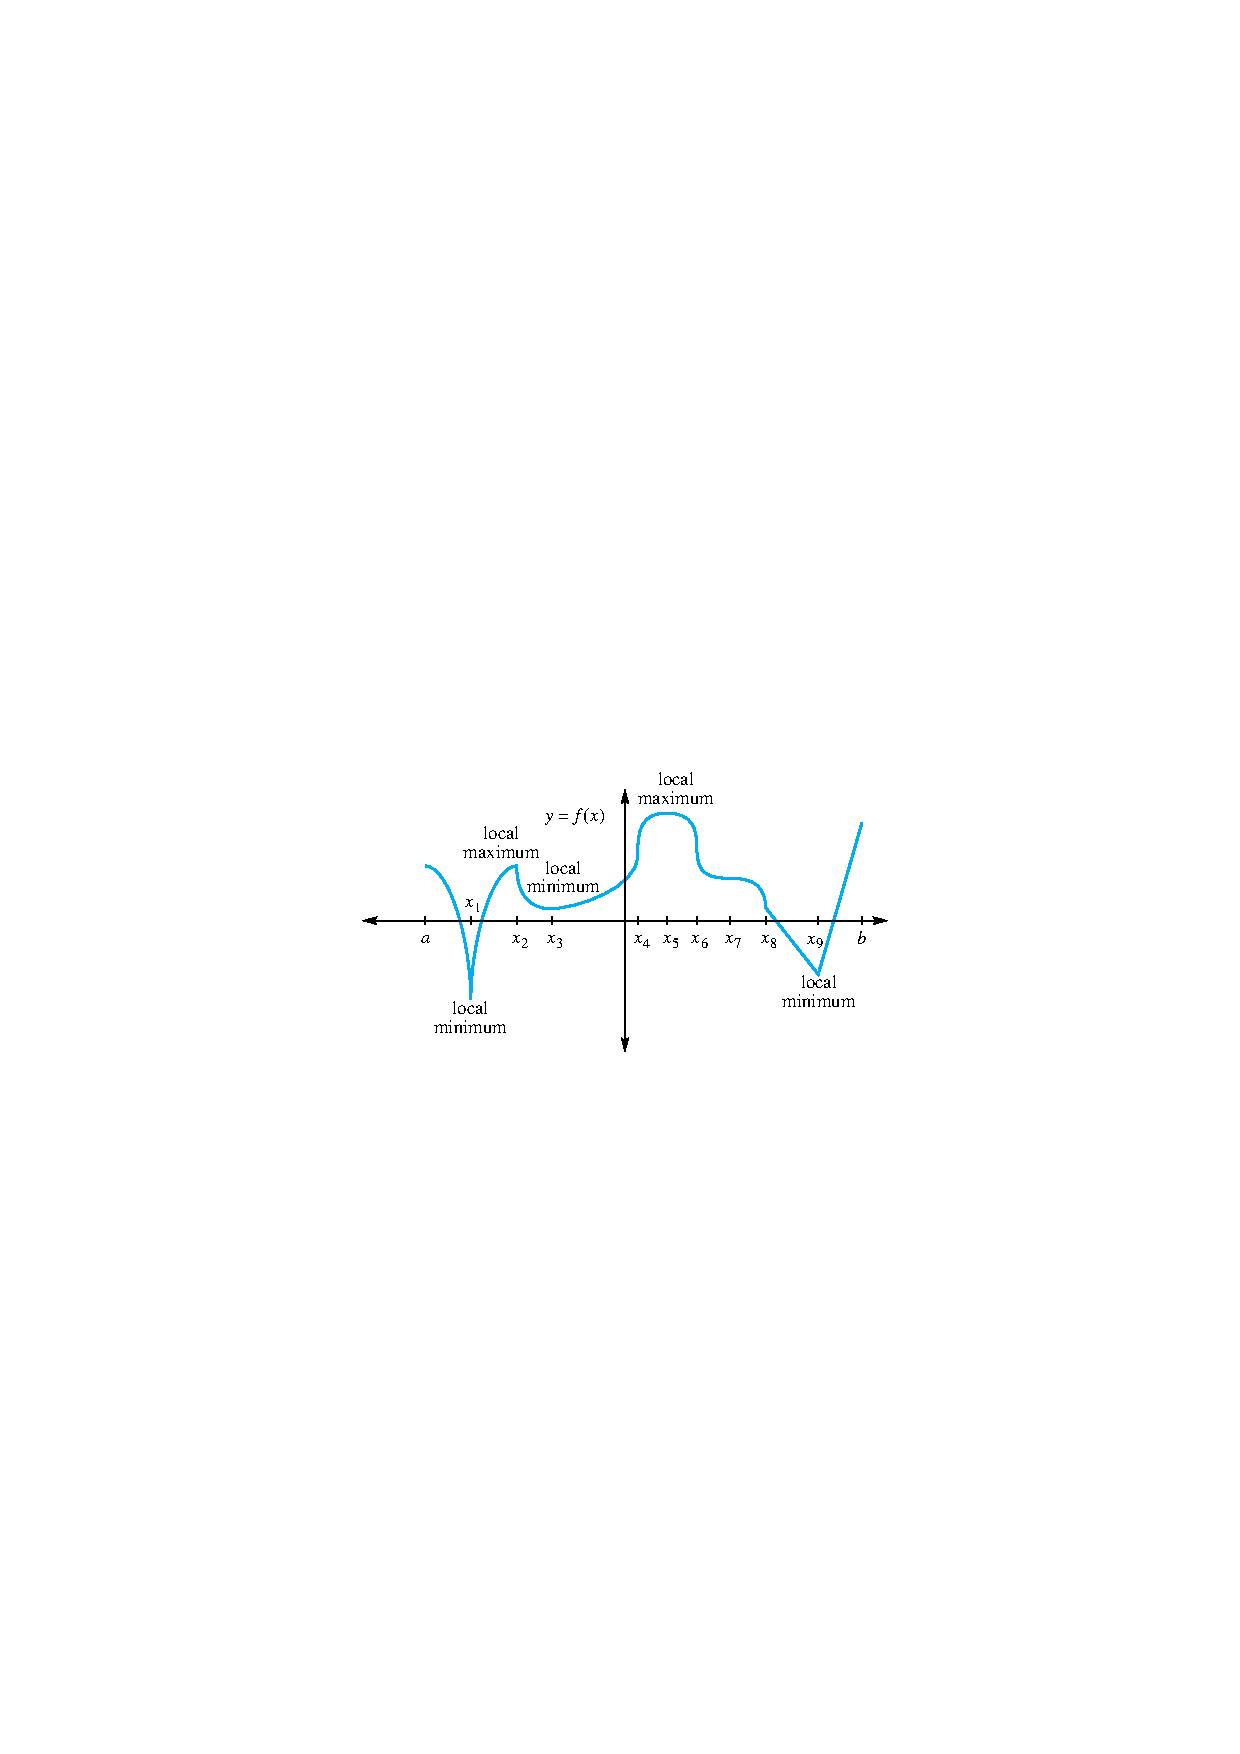
\includegraphics[width=2in]{figsamp}}
\caption{Here is the caption}
\end{figure}
\end{verbatim}
\endcode
\results
\begin{figure}[h]
\centerline{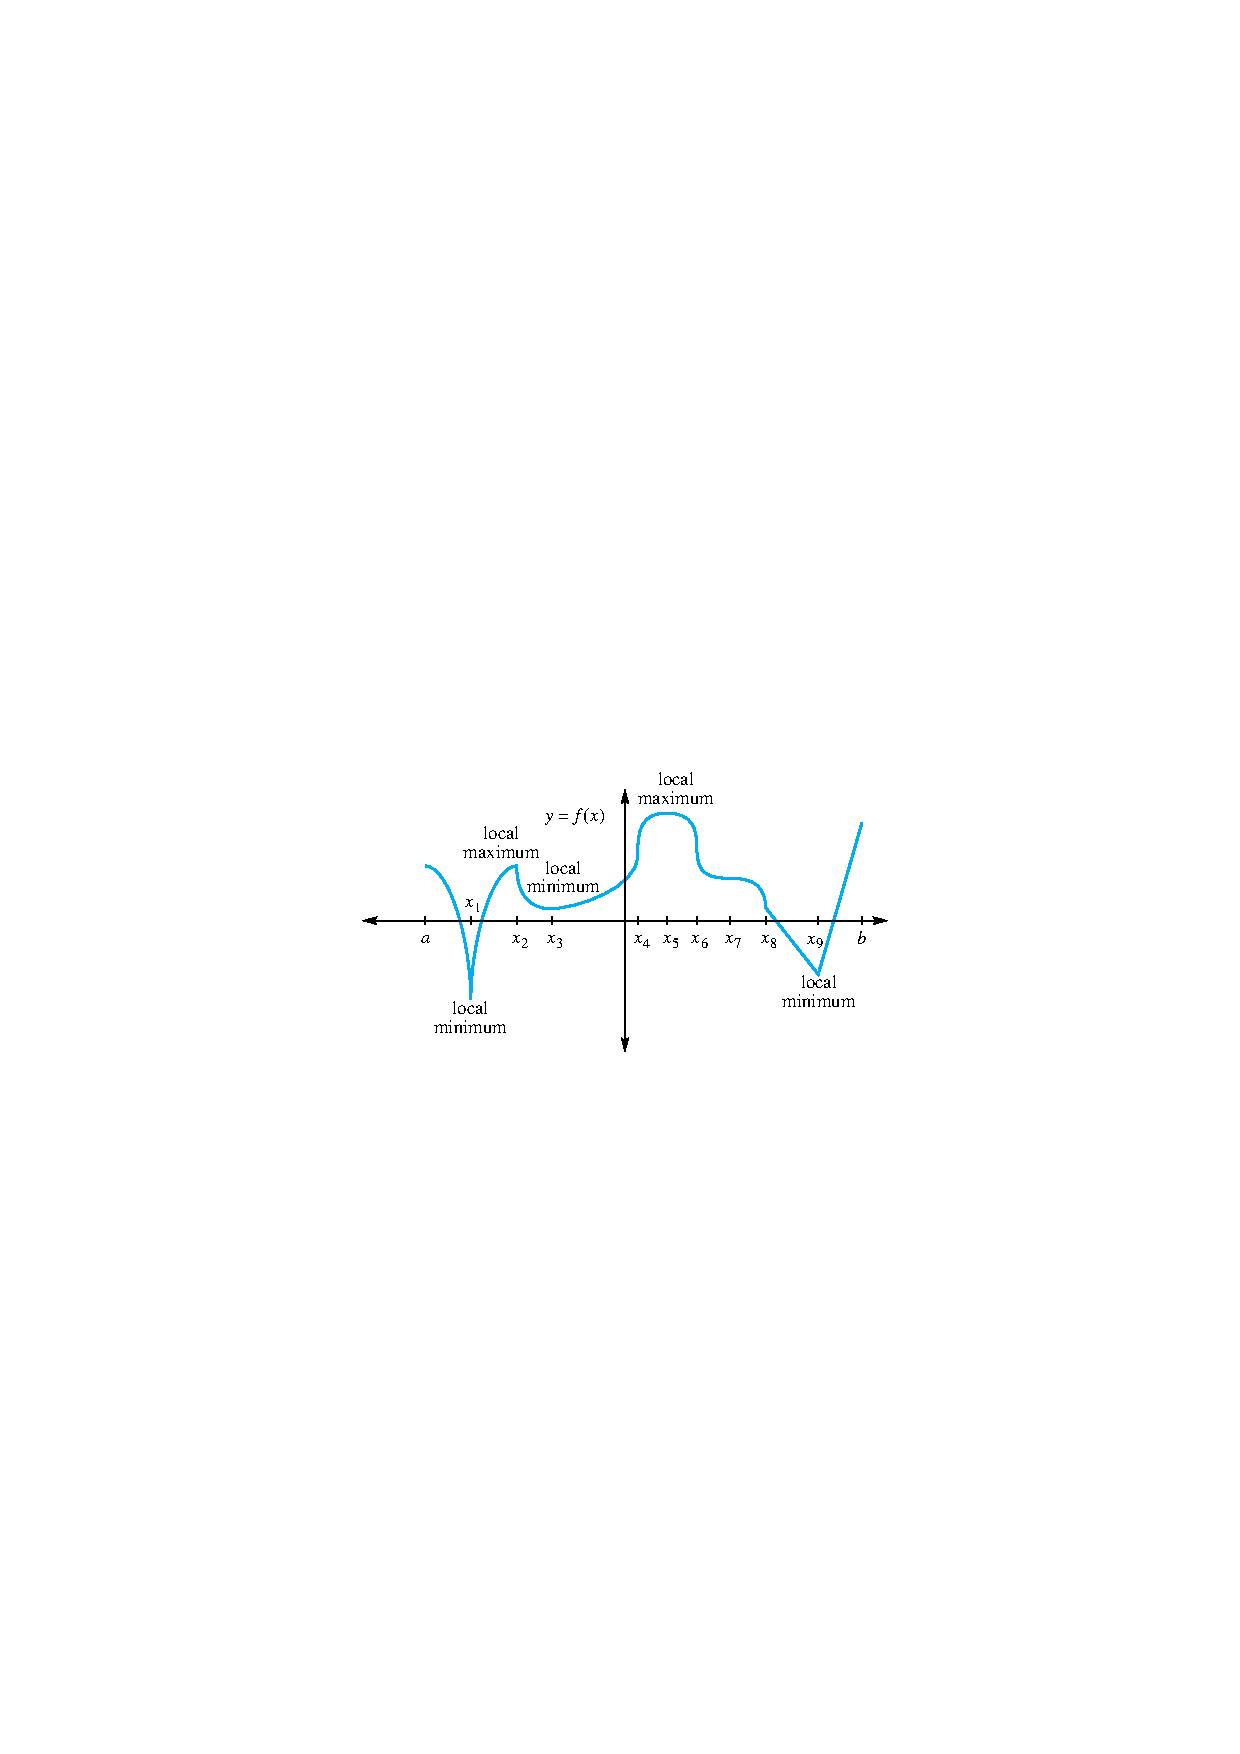
\includegraphics[width=2in]{figsamp}}
\caption{Here is the caption}
\end{figure}
\endresults


 For more information on options when using the graphicx.sty command,
\verb+\includegraphics+, please see \verb+grfguide.dvi+, which is included
 in the graphics.zip package.
\newpage

\section{Using graphicx.sty for landscape tables and figures}
\label{landscape}
If you want your figure or table to print in landscape, you
will also want them to print on their own page. This means
you should use the \verb+\begin{figure}[p]+ or 
\verb+\begin{table}[p]+.

The \verb+\rotatebox+ takes one argument which determines the
number of degrees that the box should be rotated; and the
second argument that includes a box.

To make the figure fall in the right position we use a box
whose height is the width of the page, or \verb+\textwidth+,
which we set with \verb+\vbox to \textwidth+.

The width should be the height of the page, which we set with
the command \verb+\hsize=\textheight+ within the box.

The \verb+\vfill+ command will push the contents of the box
to the bottom, which is positioned in this case on the
right side of the page.

Here is the code to make a figure print in landscape:
\code
\begin{verbatim}
\begin{figure}[p]
\rotatebox{90}{\vbox to\textwidth{
\vfill
\hsize=\textheight

\includegraphics{}
\caption{}

}}
\end{figure}
\end{verbatim}
\hrule
\endcode

Here is an actual figure to be printed in landscape:
\code
\begin{verbatim}
\begin{figure}[p]
\rotatebox{90}{\vbox to\textwidth{
\vfill
\hsize=\textheight

\centerline{\includegraphics[width=\textheight]{figsamp.eps}}

\caption[Self-Organizing Maps and Cluster Analysis]{Self-Organizing Maps and
Cluster Analysis.  Clustering of tumor gene expression data and
identification of tumor-specific molecular markers. Hierarchical clutering
(1) and a 5x5 self organizng map (b) were used to cluster 144 tumors spanning
14 tumor classes according to their gene expression patterns (c) gene
expression values for class-specific OVA markers.}}}
\end{figure}
\end{verbatim}
\hrule
\endcode

You can see how this looks on the next page.


\begin{figure}[p]
\rotatebox{90}{\vbox to\textwidth{\vfill
\hsize=\textheight
\centerline{\includegraphics[width=\textheight]{figsamp.eps}}
\caption[Self-Organizing Maps and Cluster Analysis]{
Self-Organizing Maps and Cluster Analysis.
Clustering of tumor gene expression data and identification of tumor-specific
molecular markers. Hierarchical clutering (1) and a 5x5 self organizng map (b) 
were used to cluster 144 tumors spanning 14 tumor classes according to their gene
expression patterns (c) gene expression values for class-specific OVA
markers.}}}
\end{figure}
\clearpage

\subsection{Landscape Table}
You make a table print in landscape very much as you do
for figures:

\code
\begin{verbatim}
\begin{table}[p]
\rotatebox{90}{\vbox to\textwidth{
\hsize=\textheight

\caption{}
\begin{tabular}...\end{tabular}

}}
\end{table}
\end{verbatim}
\hrule
\endcode

Here is an example landscape table:

\code
\begin{verbatim}
\begin{table}[p]
\rotatebox{90}{\vbox to\textwidth{
\hsize=\textheight
\caption{Here is a sample landscape table caption}
\def\ph{\phantom{age }}
\def\pph{\phantom{th}}
\begin{tabular*}{.9\textheight}{@{\extracolsep\fill}lccrrrcrrr}
&&\multicolumn{4}{c}{\bf Panel A}&\multicolumn{4}{c}{\bf Panel B}\cr
&&\multicolumn{4}{c}{\bf Regression A}&\multicolumn{4}{c}{\bf Regression B}\cr
\cline{3-6}\cline{7-10}\cr
...
\end{tabular*}
}}
\end{table}
\end{verbatim}
\hrule
\endcode

You'll see this table on the next page.

\begin{table}[p]
\rotatebox{90}{\vbox to\textwidth{
\hsize=\textheight
\caption{Here is a sample landscape table caption}
\def\ph{\phantom{age }}
\def\pph{\phantom{th}}
\begin{tabular*}{.9\textheight}{@{\extracolsep\fill}lccrrrcrrr}
&&\multicolumn{4}{c}{\bf Panel A}&\multicolumn{4}{c}{\bf Panel B}\cr
&&\multicolumn{4}{c}{\bf Regression A}&\multicolumn{4}{c}{\bf Regression B}\cr
\cline{3-6}\cline{7-10}\cr
%&&\multicolumn{4}{c}{\hrulefill}&\multicolumn{4}{c}{\hrulefill}\cr
\noalign{\vskip-4pt}
&\multicolumn{1}{c}{\bf\ Actual}&\multicolumn{1}{c}{\bf\ Predicted}&\multicolumn{3}{c}{\bf
Error}&
\multicolumn{1}{c}{\bf \ Predicted}&\multicolumn{3}{c}{
\bf Error}\cr
&\multicolumn{1}{c}{\bf M2}&\multicolumn{1}{c}{\bf M2}&&&&\multicolumn{1}{c}{\bf M2}\cr
\noalign{\vskip-6pt}
\cline{4-6}\cline{8-{10}}\cr
\noalign{\vskip-6pt}
\bf\ \ Year&\bf Growth&\bf Growth&\bf Growth&\multicolumn{2}{c}{\bf Cumulative}
&\bf Growth&\bf Growth&\multicolumn{2}{c}{\bf Cumulative}\cr
\cline{5-6}\cline{9-{10}}\cr
\noalign{\vskip-9pt}
&&&&\multicolumn{1}{c}{\bf Level\hbox to-12pt{}}&\multicolumn{1}{c}{\bf Percentage}&&&
\multicolumn{1}{c}{\bf Level\hbox to-12pt{}}&\multicolumn{1}{r}{\bf Percentage}\cr
&&&&\multicolumn{1}{c}{\bf (billions)\hbox to-12pt{}}&&&&
\multicolumn{1}{c}{\bf (billions)\hbox to -12pt{}}&\cr
\noalign{\vskip3pt}
\hline
\noalign{\vskip3pt}
1990Q4&4.0& 6.4& $-$2.3\ &$-$71 &  2.2\ph& 6.5&$-$2.4\pph&$-$80&2.4\ph  \cr
1991Q4&3.0& 3.6& $-$0.5\ &$-$91 &  2.7\ph & 3.3&$-$0.3\pph&$-$92&2.7\ph  \cr
1992Q4&1.8& 6.4& $-$4.5\ &$-$257 & 7.5\ph  & 5.9&$-$4.0\pph&$-$239&6.9\ph  \cr
1993Q4&1.4& 4.8& $-$3.4\ &$-$392 & 11.2\ph  & 5.0&$-$3.6\pph&$-$381&10.9\ph  \cr
1994Q4&0.6& 3.0& $-$2.4\ &$-$489 & 13.9\ph  & 2.6&$-$2.0\pph&$-$464&13.2\ph  \cr
1995Q4&3.8& 3.5& 0.3\ &$-$495  & 13.6\ph  & 4.2&$-$0.4\pph&$-$500&13.7\ph  \cr
1996Q4&4.5& 3.9& 0.5\ &$-$495  & 13.0\ph  & 4.0&$-$0.4\pph&$-$505&13.3\ph
\cr 
\noalign{\vskip10pt}
\hline
\noalign{\vskip3pt}
\multicolumn{3}{l}{Mean Error (1990\/--1996)}&
\multicolumn{4}{l}{\phantom{$-$1.7}$-$1.78}&
\multicolumn{3}{l}{\phantom{$-$}$-$1.78}\cr
\multicolumn{3}{l}{\it RMSE}&
\multicolumn{4}{l}{\phantom{$-$$-$1.7}2.52}&
\multicolumn{3}{l}{\phantom{$-$$-$}2.40}\cr
\end{tabular*}
}}
\end{table}




\newpage

\section{Making Tables}
There are two aspects of making tables with this macro package
that need to be mentioned. 

First, you need to enter commands
as you see in the section `Normal Tables' below, in order to have the
table have the correct appearance. This includes using the
command \verb+\sphline+ instead of \verb+\hline+, which will
add a little vertical space between lines, making your
table look more professional and finished.

Second, if you are making tables with vertical lines,
which you should only do if the vertical lines are crucial
to convey the information in your table, you should use
the normal \LaTeX\ command \verb+\hline+ instead of \verb+\sphline+.

\subsection{Normal Tables}
In order to make your table conform to the Kluwer Book
specification you must follow several steps.

\begin{itemize}
\item
Use \verb+\sphline+ at the top of the table,  underneath the column headers,
and at the end of the table.

\item
Please enter \verb+\it+ before each column head, to make the
column heads appear in italic.
\item
You are discouraged from using vertical lines in tables.

\item
Make your table span the full page width if possible.
\end{itemize}

The following example shows these steps being followed and the
form of the table preamble that will cause the table
to spread out to the width of the page:

\code
\begin{verbatim}
\begin{table}[h]
\caption{This is an example table caption. If there is
enough text it will form a paragraph.}
\begin{tabular*}{\hsize}{@{\extracolsep{\fill}}lcr}
\sphline
\it$\alpha\beta\Gamma\Delta$ One&\it Two&\it Three\cr
\sphline
one&two&three\cr
one&two&three\cr
\sphline
\end{tabular*}
\end{table}
\end{verbatim}
\endcode

\results

\makeatletter
\def\@captype{table}
\makeatother
\caption{This is an example table caption. If there is
enough text it will form a paragraph.}
\leftskip-12pt
\begin{tabular*}{\hsize}{@{\extracolsep{\fill}}lcr}
\sphline
\it$\alpha\beta\Gamma\Delta$ One&\it Two&\it Three\cr
\sphline
one&two&three\cr
one&two&three\cr
\sphline
\end{tabular*}

\endresults
\eject
\subsection{Making Table Notes}
Table notes are made by entering the symbol that you want
to use in math mode in a superscript. At the end of the
table, please enter the command \verb+\begin{tablenotes}+
and enter the notes, as seen below.

\code
\begin{verbatim}
\begin{table}[h]
\caption{Effects of the Two Types of Scaling Proposed by 
\protect\inx{Dennard} and Co-Workers.$^{a,b}$}
\begin{tabular*}{\textwidth}{@{\extracolsep{\fill}}lcc}\sphline
Parameter& $\kappa$ Scaling & $\kappa$, $\lambda$ Scaling\\
\sphline
Dimension&$\kappa^{-1}$&$\lambda^{-1}$\\
Voltage&$\kappa^{-1}$&$\kappa^{-1}$\\
Currant&$\kappa^{-1}$&$\lambda/\kappa^{2}$\\
\sphline
\end{tabular*}
\begin{tablenotes}
$^a$Refs.~19 and 20.

$^b\kappa, \lambda>1$.
\end{tablenotes}
\end{table}
\end{verbatim}
\vskip-12pt
\endcode
\results
\makeatletter
\def\@captype{table}
\vskip-24pt
\makeatother
\caption{Effects of the Two Types of Scaling Proposed by \protect\inx{Dennard} 
and Co-Workers.$^{a,b}$}
\noindent
\begin{tabular*}{\textwidth}{@{\extracolsep{\fill}}lcc}
\sphline
Parameter& $\kappa$ Scaling & $\kappa$, $\lambda$ Scaling\\
\sphline
Dimension&$\kappa^{-1}$&$\lambda^{-1}$\\
Voltage&$\kappa^{-1}$&$\kappa^{-1}$\\
Currant&$\kappa^{-1}$&$\lambda/\kappa^{2}$\\
\sphline
\end{tabular*}
\parindent=0pt
\begin{tablenotes}
$^a$Refs.~19 and 20.

$^b\kappa, \lambda>1$.
\end{tablenotes}
\endresults
\vskip-36pt
\vskip1sp
\subsection{Vertical Lines in Tables}
Notice in the previous examples that no vertical lines were used.
If at all possible to make your meaning clear without vertical
lines, please leave them out. 

Since we usually do not want vertical
lines in tables and we do want the horizontal lines to extend
exactly to the left and right of text, 
we must go to some extra efforts to get the vertical lines
to extend to the top and bottom of the column and to not
have extra horizontal space to the right of the vertical line
in the last column.
Remember to
add another column entry to the table preamble
and then not to use that column, as seen below. Also notice
that we use \verb+\hline+ instead of \verb+\sphline+
when making tables with vertical lines.

\vtop to 0pt{
\code
\hbox to\textwidth{%
\vtop{\hsize=.5\textwidth
\begin{verbatim}
\begin{tabular}{|c|c}\hline
 A         \\ \hline
 B         \\ \hline
\end{tabular}
\end{verbatim}}
\vtop{\vskip8pt \hsize=.5\textwidth

\centerline{Which will make a little table that looks like this:}

\centering
\begin{tabular}{|c|c}\hline
 A         \\ \hline
 B         \\ \hline
\end{tabular}
}}
\endcode
\hrule
\vss}
\newpage


\section{To Illustrate an Algorithm}

The \verb+\begin{algorithm}...\end{algorithm}+ may be used
to illustrate an algorithm.

\begin{itemize}
\item
Spaces and
blank lines will be preserved.
Math and font changes may be used. 

\item
Line beginnings may be
positioned with a \verb+\ +, which may be used as many
times as you need. A backslash followed by a space
will provide a space a bit wider than the width of 2 `M's.

\item
If you want to break lines on the screen but not break the line
in the results, use `\%' at the end of line, as you see in
the fifth line in this example.

\item
The command
\verb+\bit+ will produce bold italics if you are using PostScript fonts, 
boldface in Computer Modern. 

\item
\verb+\note{}+ will position the note on the right margin. 
\end{itemize}



\code
\begin{verbatim}
\begin{algorithm}
{\bit Evaluate-Single-FOE} ({\bf x$_f$, I$_0$, I$_1$}):
\ {\bf I}+ := {\bf I}$_1$;
\ ($\phi,\theta$) := (0,0);
\ {\it repeat}\note{/*usually only 1 interation required*/}
\ \ (s$_{opt}${\bf E}$_\eta$) := {\bit Optimal-Shift}%
  ({\bf I$_0$,I$^+$,I$_0$,x$_f$});
\ \ ($\phi^+$, $\theta^+$) := {\bit Equivalent-Rotation} ({\bf s}$_{opt}$);
\ \ ($\phi$, $\theta$) := ($\phi$, $\theta$) + ($\phi^+$, $\theta^+$);
\ \ {\bf I}$^+$:= {\bit Derotate-Image} ({\bf I}$_1$, $\phi$, $\theta$);
\ \ {\it until} ($|\phi^+|\leq\phi_{max}$ \& $|\theta^+|\leq\theta_{max}$);
\ {\it return} ({\bf I}$^+$, $\phi$, $\theta$, E$_\eta$).
End pseudo-code.
\end{algorithm}
\end{verbatim}
\endcode

\results
\begin{algorithm}
{\bit Evaluate-Single-FOE} ({\bf x$_f$, I$_0$, I$_1$}):
\ {\bf I}+ := {\bf I}$_1$;
\ ($\phi,\theta$) := (0,0);
\ {\it repeat}\note{/*usually only 1 interation required*/}
\ \ (s$_{opt}${\bf E}$_\eta$) :={\bit Optimal-Shift} %
  ({\bf I$_0$,I$^+$,I$_0$,x$_f$});
\ \ ($\phi^+$, $\theta^+$) := {\bit Equivalent-Rotation} ({\bf s}$_{opt}$);
\ \ ($\phi$, $\theta$) := ($\phi$, $\theta$) + ($\phi^+$, $\theta^+$);
\ \ {\bf I}$^+$:= {\bit Derotate-Image} ({\bf I}$_1$, $\phi$, $\theta$);
\ \ {\it until} ($|\phi^+|\leq\phi_{max}$ \& $|\theta^+|\leq\theta_{max}$);
\ {\it return} ({\bf I}$^+$, $\phi$, $\theta$, E$_\eta$).
End pseudo-code.
\end{algorithm}
\endresults

\clearpage


\newpage
\section{End of Article}
Getting the end of article commands in the right order will not
be difficult if you use the {\tt procsamp.tex} template file.
The commands should be used in this order:
Acknowledgments (optional), Appendix (optional), References, and 
finally \verb+\end{article}+.

\code
\begin{verbatim}
%% End of article:

%% optional:
% \begin{glossary}
% \end{glossary}

%% optional:
%\begin{acknowledgements}
%\end{acknowledgements}

%% optional: 
%\chapappendix{<Optional Chapter Appendix Letter or title>}
%\chapappendix{} % Untitled chapter appendix

\begin{references}
...
\end{references}

\end{article}
\end{document}
\end{verbatim}
\hrule

\newpage
\section{Glossary}
An optional glossary section is available. Its commands are
very straightforward:\label{gloss}

\begin{verbatim}
\begin{glossary}
\term{xxx}Text...
\term{yyy}Text...
\end{glossary}
\end{verbatim}

Here is an example:

\code
\begin{verbatim}
\begin{glossary}
\term{GaAs}Gallium Arsinide. For similar device sizes GaAs transistors 
have three to
five times greater transconductance than those of of silicon bipolar
and MOS transistors.

\term{VLSI}Very Large Scale Integration. Since the mid-1970's 
VLSI technology has been successfully used in many areas, but its effect on
computers of all shapes and sizes has been the most dramatic. Some of the
application areas got boosts in performance while others became
feasible.

\end{glossary}
\end{verbatim}
\endcode
\results
\begin{glossary}
\term{GaAs}Gallium Arsinide. For similar device sizes GaAs transistors 
have three to
five times greater transconductance than those of of silicon bipolar
and MOS transistors.

\term{VLSI}Very Large Scale Integration. Since the mid-1970's 
VLSI technology has been successfully used in many areas, but its effect on
computers of all shapes and sizes has been the most dramatic. Some of the
application areas got boosts in performance while others became
feasible.

\end{glossary}
\vskip-12pt
\endresults

\vskip-12pt
\vskip1sp
\subsection{Acknowledgements}

\vtop to 0pt{
\code
\begin{verbatim}
\begin{acknowledgments}
We would like to thank....
\end{acknowledgments}
\end{verbatim}
\endcode
\results
\vskip-1.5\baselineskip
\vskip1sp
\begin{acknowledgments}
We would like to thank....
\end{acknowledgments}
\endresults
\vss}
\newpage



\section{Appendices}
There are two sets of appendix commands; those for the end of
the chapter and those for an appendix at the end of the book.
\subsection{End of Chapter Appendix}
An appendix to appear at the end of the book
is
made with the command \verb+\appendix{}+, as seen below.
If you want only one appendix, follow \verb+\appendix+ with facing
curly brackets: \verb+\appendix{}+.

Section numbers, equation numbers, and captions will all use the 
appendix letter as well as their number. Each new appendix will
generate a new appendix letter.

Here are some appendix possibilities:
\code
\begin{verbatim}
\chapappendix{This is a Chapter Appendix}
This is an appendix which is meant to appear in individual chapters
of the proceedings, not at the end of the book.

\begin{equation}
g_i(y|f)=\sum_x P(x|F_n)f_i(y|x)
\end{equation}

\chapappendix{}
This is a chapter appendix without a title
which is meant to appear in individual chapters
of the proceedings, not at the end of the book.

\begin{equation}
g_i(y|f)=\sum_x P(x|F_n)f_i(y|x)
\end{equation}
\end{verbatim}
\endcode

\results
\chapappendix{This is a Chapter Appendix}
This is an appendix which is meant to appear in individual chapters
of the proceedings, not at the end of the book.

\begin{equation}
g_i(y|f)=\sum_x P(x|F_n)f_i(y|x)
\end{equation}

\chapappendix{}
This is a chapter appendix without a title
which is meant to appear in individual chapters
of the proceedings, not at the end of the book.

\begin{equation}
g_i(y|f)=\sum_x P(x|F_n)f_i(y|x)
\end{equation}
\endresults
\newpage
Here is a longer example showing a figure, table and equation
in the appendix:

\code
\vskip-12pt
\vskip1sp
\begin{verbatim}
\begin{figure}[h]
\caption{This is an appendix figure caption.}
\end{figure}

\begin{table}[h]
\caption{This is an appendix table caption.}
\centering
\begin{tabular}{ccc}
\hline
one&two&three\\
\hline
C&D&E\\
\hline
\end{tabular}
\end{table}

\begin{equation}
\alpha\beta\Gamma\Delta
\end{equation}

\chapappendix{}
This is a chapter appendix without a title ...
\end{verbatim}
\endcode

\results
\vskip-24pt
\vskip1sp
\let\section\savesection

\chapappendix{This is a Chapter Appendix}
This is an appendix which is meant to appear in individual chapters
of the proceedings, not at the end of the book.

\begin{figure}[h]
\caption{This is an appendix figure caption.}
\end{figure}

\vskip-24pt
\vskip1sp
\begin{table}[h]
\caption{This is an appendix table caption.}
\centering
\begin{tabular}{ccc}
\hline
one&two&three\\
\hline
C&D&E\\
\hline
\end{tabular}
\end{table}
\begin{equation}
\alpha\beta\Gamma\Delta
\end{equation}


\chapappendix{}
This is a chapter appendix without a title 
meant to appear in individual chapters
of the proceedings, not at the end of the book.
\begin{equation}
e=mc^2
\end{equation}
\endresults


\section{End Notes and Footnotes}
In this style the default is end notes rather than footnotes. The
user enters the usual footnote command \verb+\footnote{<text>}+.
A number appears in the text as it would with a footnote, but
with this style the note only appears at the end of the chapter
when the user writes \verb+\notes+.

\code
\begin{verbatim}
Here is some sample text\footnote{Here is our first sample note}
to show how end notes print.

\notes
\end{verbatim}
\endcode
\results
\global\footnum=0
Here is some sample text\footnote{Here is our first sample note}
to show how end notes print.

\notes
\endresults

\subsection{If you want Footnotes instead of Endnotes}
If you would rather have footnote at the bottom of the page,
you may write this command below the documentstyle or documentclass
command: \verb+\let\footnote\savefootnote+.

If you would also like to have a ruled line appear above the
footnote, you may write this: 

\noindent
\verb+\let\footnoterule\savefootnoterule+.
\newpage

\section{References}

Before \verb+\begin{document}+ in your proctmpl.tex file you will see the
following information:

\begin{verbatim}
% Bibliography Style Settings:
% ============================
% Choose either kluwerbib or normallatexbib:

%%%
\kluwerbib % will produce this kind of bibliography entry:

%  Anderson, Terry L.,...
%    continuing bib entry here

%  \cite{xxx} will print without brackets around the citation.
% \bibliographystyle{kapalike} % should be used when you use \verb+\kluwerbib+.

%%%
%\normallatexbib %will produce bibliography entries as shown in the
                % LaTeX book

% [1] Anderson, Terry L.,
%     continuing bib entry

% \cite{xxx} will print with square brackets around the citation, i.e., [1].

% Any \verb+\bibliographystyle{}+ may be used with \verb+\normallatexbib+, but
% you should check with your editor to find the style preferred for
% your book.

% Change Brackets around Citation:
% ================================

%% Default with \kluwerbib is no brackets around citation. 
%% Default with \normallatexbib is square brackets around citation. 

% For parens around citation uncomment these:

%\let\lcitebracket(
%\let\rcitebracket)

% For square brackets around citation uncomment these:

%\let\lcitebracket[
%\let\rcitebracket]

%%%%%%%  <<== End Bibliography Style Settings
\end{verbatim}

\newpage
\section{Using the Kluwerbib or Normallatexbib Bibliography Option}
Unless you have a preference to use the normal \LaTeX\ bibliography
styles, you should leave \verb+\kluwerbib+ uncommented.

If you
plan on using the \verb+\cite{}+ command,
and are using \verb+\kluwerbib+,
remember that \verb+\bibitem+ should be used with the square bracket argument.
With \verb+\kluwerbib+,
whatever is typed between square brackets after \verb+\bibitem+
will be printed when you use \verb+\cite{}+.


When the square bracket argument is used:

\code
\begin{verbatim}
Here is our citation: \cite{lacey}.
...
\bibitem[Lacey, 1968]{lacey}
Lacey, W.K. (1968). {\it History of Socialism}. Ithaca, NY: Cornell
University Press.
\end{verbatim}
\endcode
\results
Here is our citation: Lacey, 1968.
\endresults

If you forgot to use the square bracket argument, you will get
the name of the symbolic label when you type \verb+\cite{}+, i.e.,

\code
\begin{verbatim}
Here is our citation: \cite{lacey}.
...
\bibitem{lacey}
Lacey, W.K. (1968). {\it History of Socialism}. Ithaca, NY: Cornell
University Press.
\end{verbatim}
\endcode
\results
Here is our citation: lacey.
\endresults

When using the \verb+\normallatexbib+ option, you don't have
to use the square bracket argument, since the bibitems will
be numbered and \verb+\cite+ will produce numbers.
\newpage

\subsection{chapthebibliography}
Now you can use the \verb+\begin{chapthebibliography}{<widest bib entry>}+
command, which works like the \newline
\verb+\begin{thebibliography}{<widest bib entry>}+ command, except
that it can be used at the end of chapters.

Here is how bib entries will be formatted if you have uncommented the 
\verb+\kluwerbib+ command near the top of the file. 

\code
\begin{verbatim}
\kluwerbib %% <== above \begin{document}
...
Sample citations: \cite{lacey,oliva}.

\begin{chapthebibliography}{}
\bibitem[Anderson, et al]{ander}
Anderson, Terry L., and Fred S. McChesney. (n.d.). ``Raid or Trade?
An Economic Model of Indian-WhiteRelations,'' Political Economy Research
Center Working Paper 93--1.

\bibitem[Lacey, 1968]{lacey}
Lacey, W.K. (1968). {\it History of Socialism}. Ithaca, NY: Cornell
University Press.

\bibitem[Oliva, 1971]{oliva}
Oliva, Pavel. (1971). {\it Sparta and Her Social Problems.} Amsterdam: Adolf
M. Hakkert.

\bibitem[Zimmern, 1961]{zimmern}
Zimmern, Alfred. (1961). {\it The Greek Commonwealth: Politics and Economics
in Fifth-Century Athens,}\/ 5th ed. New York: Galaxy Book, Oxford University
Press.
\end{chapthebibliography}
\end{verbatim}
\endcode
\results
\kluwerbib
Sample citations: Lacey, 1968, Oliva, 1971.

\begin{chapthebibliography}{}
\bibitem[Anderson, et al]{aander}
Anderson, Terry L., and Fred S. McChesney. (n.d.). ``Raid or Trade?
An Economic Model of Indian-WhiteRelations,'' Political Economy Research
Center Working Paper 93--1.

\bibitem{alacey}
Lacey, W.K. (1968). {\it History of Socialism}. Ithaca, NY: Cornell
University Press.

\bibitem[Oliva, 1971]{aoliva}
Oliva, Pavel. (1971). {\it Sparta and Her Social Problems.} Amsterdam: Adolf
M. Hakkert.

\bibitem[Zimmern, 1961]{azimmern}
Zimmern, Alfred. (1961). {\it The Greek Commonwealth: Politics and Economics
in Fifth-Century Athens,}\/ 5th ed. New York: Galaxy Book, Oxford University
Press.
\end{chapthebibliography}
\endresults
\newpage
If you use 
\verb+\normallatexbib+  your bibliography will
format just as it would with a standard \LaTeX\ style.

\code
\begin{verbatim}
\normallatexbib %% <== above \begin{document}
...
Sample citations: \cite{raidtrade,sparta}.

\begin{chapthebibliography}{1}
\bibitem{raidtrade}
Anderson, Terry L., and Fred S. McChesney. (n.d.). ``Raid or Trade?
An Economic Model of Indian-WhiteRelations,'' Political Economy Research
Center Working Paper 93--1.

\bibitem{history}
Lacey, W.K. (1968). {\it History of Socialism}. Ithaca, NY: Cornell
University Press.

\bibitem{sparta}
Oliva, Pavel. (1971). {\it Sparta and Her Social Problems.} Amsterdam: Adolf
M. Hakkert.

\bibitem{earlygreek}
Zimmern, Alfred. (1961). {\it The Greek Commonwealth: Politics and Economics
in Fifth-Century Athens,}\/ 5th ed. New York: Galaxy Book, Oxford University
Press.
\end{chapthebibliography}
\end{verbatim}
\endcode
\results
\normallatexbib
Sample citations: [1,3].

\begin{chapthebibliography}{1}
\bibitem{raidtradey}
Anderson, Terry L., and Fred S. McChesney. (n.d.). ``Raid or Trade?
An Economic Model of Indian-WhiteRelations,'' Political Economy Research
Center Working Paper 93--1.

\bibitem{historyy}
Lacey, W.K. (1968). {\it History of Socialism}. Ithaca, NY: Cornell
University Press.

\bibitem{spartay}
Oliva, Pavel. (1971). {\it Sparta and Her Social Problems.} Amsterdam: Adolf
M. Hakkert.

\bibitem{earlygreeky}
Zimmern, Alfred. (1961). {\it The Greek Commonwealth: Politics and Economics
in Fifth-Century Athens,}\/ 5th ed. New York: Galaxy Book, Oxford University
Press.
\end{chapthebibliography}
\endresults

\newpage
Using symbolic names for your bibliography is done as you see
below, using the \verb+\normallatexbib+ command.

\code
\begin{verbatim}
Sample citations: \cite{xraidtrade,xsparta}.

\begin{chapthebibliography}{AnderMcC}
\bibitem[AnderMcC]{xraidtrade}
Anderson, Terry L., and Fred S. McChesney. (n.d.). ``Raid or Trade?
An Economic Model of Indian-WhiteRelations,'' Political Economy Research
Center Working Paper 93--1.

\bibitem[Lacey68]{xhistory}
Lacey, W.K. (1968). {\it History of Socialism}. Ithaca, NY: Cornell
University Press.

\bibitem[Oliva71]{xsparta}
Oliva, Pavel. (1971). {\it Sparta and Her Social Problems.} Amsterdam: Adolf
M. Hakkert.

\bibitem[Zim61]{xearlygreek}
Zimmern, Alfred. (1961). {\it The Greek Commonwealth: Politics and Economics
in Fifth-Century Athens,}\/ 5th ed. New York: Galaxy Book, Oxford University
Press.
\end{chapthebibliography}
\end{verbatim}
\endcode

\results
Sample citations: [AnderMcC; Oliva71].

\begin{chapthebibliography}{AnderMcC}
\bibitem[AnderMcC]{zraidtrade}
Anderson, Terry L., and Fred S. McChesney. (n.d.). ``Raid or Trade?
An Economic Model of Indian-WhiteRelations,'' Political Economy Research
Center Working Paper 93--1.

\bibitem[Lacey68]{zhistory}
Lacey, W.K. (1968). {\it History of Socialism}. Ithaca, NY: Cornell
University Press.

\bibitem[Oliva71]{zsparta}
Oliva, Pavel. (1971). {\it Sparta and Her Social Problems.} Amsterdam: Adolf
M. Hakkert.

\bibitem[Zim61]{xearlygreek}
Zimmern, Alfred. (1961). {\it The Greek Commonwealth: Politics and Economics
in Fifth-Century Athens,}\/ 5th ed. New York: Galaxy Book, Oxford University
Press.
\end{chapthebibliography}
\endresults
\newpage


\subsection{Changing the bracket around the citation}
If you want to set the bracket around the citation to parens,
you can do it at the top of your file:

\begin{verbatim}
%%%%%%% To change brackets around citation ==>>
% Default with \kluwerbib is no brackets around citation. 
% Default with \normallatexbib is square brackets around citation. 

%If you want parens, around citation, i.e., (citation), uncomment these lines:
\let\lcitebracket(
\let\rcitebracket)
\end{verbatim}

Then the citation will look like:

\code
\begin{verbatim}
\let\lcitebracket(
\let\rcitebracket)
...
Sample citations: \cite{xraidtrade,xsparta}.
\end{verbatim}
\endcode
\results
Sample citations: (AnderMcC,Oliva71).
\endresults


\newpage
\section{Using BibTeX for your Chapter References}
Using BibTeX is a bit more effort, but the major advantage
is that you can build a database of your references
that you can reuse for other books or articles.

To use Bib\TeX\ to make your chapter bibliography
you will follow the usual \LaTeX\ method, but you
must also use two new commands: {\tt\string\chapbblname} and
{\tt\string\chapbibliography}, along with the familiar
{\tt\string\bibliographystyle{}}. 

The {\tt\string\chapbblname}
command is needed to let LaTeX know which .bbl file to
use since there will be presumably more than one bibliography
in the complete book. The {\tt\string\chapbibliography} command 
makes the bibliography print in the style
appropriate to a bibliography appearing in a chapter.

\begin{verbatim}
\bibliographystyle{<name of a .bst file>} % Choose the BibTeX style

\chapbblname{<name of a .bbl file>} 
              % The .bbl file appears after you run BibTeX
              % on your file; its name will be the same as the 
              % file name, but with a .bbl extension
				      
\chapbibliography{<name of one or more .bib files>}
              % .bib files are the bibliography database
\end{verbatim}                            
\vskip-12pt
Follow these steps.

\def\dothis#1#2{\vskip-8pt\vskip1sp
\item[\bf#1.]{\bf\uppercase{#2}}}
\begin{enumerate}
\parskip=4pt
\item[\bf1.]{\bf\uppercase{Preparation}}

\vskip6pt
{\bf Make a .bib file}

If you do not already have one or more .bib files, 
make a {\tt xxx.bib} file, with `{\tt xxx}' being any file name you choose.
The .bib file or files are a database of references.
Please see Leslie Lamport's {\it \LaTeX\ A Document Preparation System}
for information on the form of entries in the .bib file.

\vskip6pt
{\bf Enter Citations}

Write either \verb+\cite{<label>}+ or \verb+\nocite{<label>}+
for each reference that you want to appear in the bibliography.
The name of the \verb+<label>+ is found in the .bib file.

Each citation pull an entry from the .bib file with the same
label name and make it appear in the bibliography.

There is also a command called
\verb+\nocite+ which is used in the same way as \verb+\cite+
but will not print a citation. Its only purpose is to
cause the matching entry to be pulled from the database
and added to the .bbl file when BibTeX is run on the .tex file.

For example:
\begin{verbatim}
Here are some more citations
\cite{dms80}, \cite{gm91}, \cite{hhmz77,hb85},
\cite{kt78}. \nocite{kl94}
\end{verbatim}
\null
\vskip1sp
\dothis{2}{Commands to enter in your .tex file}



\vskip6pt
{\bf Supply a Bibliography Style}

Use kapalike or alpha for the bibliographystyle:

\vskip3pt
{\tt\string\bibliographystyle\string{kapalike\string}}
\vskip3pt

The kapalike.bst file may be downloaded from the Kluwer ftp site,
in the same directory as you found the other book files: \\
{\tt http://www.wkap.nl/authors/bookstylefiles/latexstyles}.

Please put kapalike.bst in the same directory where you are working, or in
a directory where BibTeX can find it when it is running.

\vskip6pt
{\bf Supply a .bbl file name}

Write \verb+\chapbblname{<name of your bbl file>}+\hfill\break
with the name of your bbl file being the name of the file
you are writing, i.e, if you are working in a file named
chap1.tex, the name you should supply is 
\vskip-12pt
\vskip1sp
\begin{verbatim}
\chapbblname{chap1}
\end{verbatim}
\vskip-12pt

{\bf  Supply a .bib file name, or names}

Next you must write \verb+\chapbibliography{xxx}+, 
with `xxx' being the name of 
the .bib database file that you have written. You can also use more
than one .bib file, in which case you must separate the filenames with
a comma: \verb+\chapbibliography{xxx,yyy}+.

For example:
\vskip-12pt
\vskip1sp
\begin{verbatim}
\bibliographystyle{kapalike}
\chapbblname{chap1}
\chapbibliography{bkbib}
\end{verbatim}

\vskip-1pt
\null
\dothis{3}{Making the .bbl file}

{\bf Run LaTeX on your file}

Once the citations are entered in your text, you can
run LaTeX on the file. This step is needed to send
label information to the .aux file, which will tell BibTeX
which entries should be taken from the .bib database and
used in the .bbl file that it will make.
\vskip6pt

{\bf Run BibTeX on your file to produce a .bbl file}

Use the BibTeX program to make the .bbl file, by entering
the command \verb+bibtex filename+ with filename being
the .tex file you are working on, without the .tex extension.

If the .tex file is named chap1.tex 
you will produce a file named chap1.bbl.
\vskip6pt
{\bf Run \LaTeX\ on your file two more times}

After you have a .bbl file, you should
run LaTeX on your .tex file to produce
a formatted bibliography. 

The next time you run \LaTeX\ on your file your citations
will appear.
(You must run LaTeX on the file one final time so
that the entries in the bibliography are able
to send information about the text of the citations
to the .aux file.)
\null
\vskip6pt
\vskip6pt
\vskip6pt
\dothis{4}{Sending in the bbl file}

You have two choices at this point: 

1) Either send the .bbl
file in to the editor at the same time that you submit
your chapter, or 

2) Copy the \verb+\bibitem+s from your .bbl file and drop
them into a \verb+\chapthebibliography+ environment. If
you follow this path, you will no longer need the
commands you originally entered, \verb+\bibliographystyle{}+,
\verb+\chapbblname{}+, or \verb+\chapbibliography{}+.
This option may be preferable in that there is greater
assurance that
the .bbl file will not become separated from the
.tex file.

\vtop to 0pt{
\vskip-18pt
\vskip1sp
\begin{verbatim}
\begin{chapbibliography}
<add bibitems here>
\end{chapbibliography}
\end{verbatim}
\vss}
\end{enumerate}
\eject


\section{Commands for the end of the Book: End Matter}
The end of the book should use this order:
\begin{verbatim}
Glossary %% optional
Appendices %% optional
Bibliography
Index
\end{verbatim}

\subsection{Glossary}
You've seen how to format a glossary on page \pageref{gloss}.
If you make the glossary at the end of a chapter or at the
end of the book the commands are identical.

\subsection{End of book appendix}
\setcounter{alphanum}{0}
The appendix commands at the end of the book are exactly
the same, except that they use \verb+\appendix{}+ instead
of \verb+\chapappendix{}+.

If you want only one appendix, follow \verb+\appendix+ with facing
curly brackets: \verb+\appendix{}+.

Section numbers, equation numbers, and captions will all use the 
appendix letter as well as their number. Each new appendix will
generate a new appendix letter.

Here are some appendix possibilities:
\code
\begin{verbatim}
\appendix{}
This is an appendix.
\begin{equation}\sum_k P(k) \sum_i \sum_y f_i(y|k)^2\end{equation}

\appendix{Pspace $\supseteq$ PCP(log n)}
....
\end{verbatim}
\endcode
\global\let\savenewpage\newpage

\results
\let\section\savesection
\appendix{}
This is an appendix.
\begin{equation}\sum_k P(k) \sum_i \sum_y f_i(y|k)^2\end{equation}

\appendix{Pspace $\supseteq$ PCP(log n)}
This is an appendix.
\begin{equation}
\sum_k P(k) \sum_i \sum_y f_i(y|k)^2
\end{equation}
\endresults

\newpage
\subsection{Bibliography at end of Book}
The commands \verb+\begin{thebibliography}{<widest label>}+...
\verb+\end{thebibliography}+ may be used to format the
bibliography at the end of the book.

The appearance of the bibliography will differ depending on
whether \verb+\kluwerbib+ or \verb+\normallatexbib+ has
been uncommented at the beginning of the file.

If you
plan on using the \verb+\cite{}+ command,
and are using \verb+\kluwerbib+,
remember that \verb+\bibitem+ should be used with the square bracket argument.
With \verb+\kluwerbib+,
whatever is typed between square brackets after \verb+\bibitem+
will be printed when you use \verb+\cite{}+.

\subsection{Using thebibliography}
You can use the \LaTeX\ command 
\verb+\begin{thebibliography}{<widest label>}+ at the end of
the book, and use \verb+\bibitem+ with or without the optional
argument in square brackets. The appearance will differ depending
on whether you uncommented \verb+\kluwerbib+ or \verb+\normallatexbib+
at the beginning of the file.

\code
\begin{verbatim}
\kluwerbib %% <== above \begin{document}
...
\begin{thebibliography}{}
\bibitem[Anderson, et al]{ander}
Anderson, Terry L., and Fred S. McChesney. (n.d.). ``Raid or Trade?
An Economic Model of Indian-WhiteRelations,'' Political Economy Research
Center Working Paper 93--1.

\bibitem[Lacey, 1968]{lacey}
Lacey, W.K. (1968). {\it History of Socialism}. Ithaca, NY: Cornell
University Press.

\bibitem[Oliva, 1971]{oliva}
Oliva, Pavel. (1971). {\it Sparta and Her Social Problems.} Amsterdam: Adolf
M. Hakkert.
\end{thebibliography}
\end{verbatim}
\endcode
\results
\kluwerbib
\let\chapter\savechapter
\begin{thebibliography}{}
\bibitem{ander}
Anderson, Terry L., and Fred S. McChesney. (n.d.). ``Raid or Trade?
An Economic Model of Indian-WhiteRelations,'' Political Economy Research
Center Working Paper 93--1.

\bibitem{lacey}
Lacey, W.K. (1968). {\it History of Socialism}. Ithaca, NY: Cornell
University Press.

\bibitem{oliva}
Oliva, Pavel. (1971). {\it Sparta and Her Social Problems.} Amsterdam: Adolf
M. Hakkert.

\end{thebibliography}
\endresults

\newpage
When you have used
\verb+\normallatexbib+ your bibliography will
format just as it would with a standard \LaTeX\ style.

\code
\begin{verbatim}
\normallatexbib %% <== above \begin{document}
...
\begin{thebibliography}{1}
\bibitem{raidtrade}
Anderson, Terry L., and Fred S. McChesney. (n.d.). ``Raid or Trade?
An Economic Model of Indian-WhiteRelations,'' Political Economy Research
Center Working Paper 93--1.

\bibitem{history}
Lacey, W.K. (1968). {\it History of Socialism}. Ithaca, NY: Cornell
University Press.

\bibitem{sparta}
Oliva, Pavel. (1971). {\it Sparta and Her Social Problems.} Amsterdam: Adolf
M. Hakkert.

\bibitem{earlygreek}
Zimmern, Alfred. (1961). {\it The Greek Commonwealth: Politics and Economics
in Fifth-Century Athens,}\/ 5th ed. New York: Galaxy Book, Oxford University
Press.
\end{thebibliography}
\end{verbatim}
\endcode
\results
\let\chapter\savechapter
\normallatexbib

\begin{thebibliography}{1}
\bibitem{raidtradea}
Anderson, Terry L., and Fred S. McChesney. (n.d.). ``Raid or Trade?
An Economic Model of Indian-WhiteRelations,'' Political Economy Research
Center Working Paper 93--1.

\bibitem{historya}
Lacey, W.K. (1968). {\it History of Socialism}. Ithaca, NY: Cornell
University Press.

\bibitem{spartaa}
Oliva, Pavel. (1971). {\it Sparta and Her Social Problems.} Amsterdam: Adolf
M. Hakkert.

\bibitem{earlygreeka}
Zimmern, Alfred. (1961). {\it The Greek Commonwealth: Politics and Economics
in Fifth-Century Athens,}\/ 5th ed. New York: Galaxy Book, Oxford University
Press.
\end{thebibliography}
\endresults

\newpage
If you want to use a symbolic name for your references, please
use \verb+\normallatexbib+, and the symbolic name in square
brackets after \verb+\bibitem+:

\code
\begin{verbatim}
\begin{thebibliography}{AnderMcC}
\bibitem[AnderMcC]{raidtrade}
Anderson, Terry L., and Fred S. McChesney. (n.d.). ``Raid or Trade?
An Economic Model of Indian-WhiteRelations,'' Political Economy Research
Center Working Paper 93--1.

\bibitem[Lacey68]{history}
Lacey, W.K. (1968). {\it History of Socialism}. Ithaca, NY: Cornell
University Press.

\bibitem[Oliva71]{sparta}
Oliva, Pavel. (1971). {\it Sparta and Her Social Problems.} Amsterdam: Adolf
M. Hakkert.

\bibitem[Zim61]{earlygreek}
Zimmern, Alfred. (1961). {\it The Greek Commonwealth: Politics and Economics
in Fifth-Century Athens,}\/ 5th ed. New York: Galaxy Book, Oxford University
Press.
\end{thebibliography}
\end{verbatim}
\endcode
\results
\normallatexbib
\let\chapter\savechapter
\begin{thebibliography}{AnderMcC}
\bibitem[AnderMcC]{yraidtrade}
Anderson, Terry L., and Fred S. McChesney. (n.d.). ``Raid or Trade?
An Economic Model of Indian-WhiteRelations,'' Political Economy Research
Center Working Paper 93--1.

\bibitem[Lacey68]{yhistory}
Lacey, W.K. (1968). {\it History of Socialism}. Ithaca, NY: Cornell
University Press.

\bibitem[Oliva71]{ysparta}
Oliva, Pavel. (1971). {\it Sparta and Her Social Problems.} Amsterdam: Adolf
M. Hakkert.

\bibitem[Zim61]{yearlygreek}
Zimmern, Alfred. (1961). {\it The Greek Commonwealth: Politics and Economics
in Fifth-Century Athens,}\/ 5th ed. New York: Galaxy Book, Oxford University
Press.
\end{thebibliography}
\endresults

\newpage


\subsection{Using Bib\TeX\ for References for End of Book}
The same series of steps that were described earlier to
make a chapter bibliography are also followed to make
a Bib\TeX\ bibliography at the end of the book. The
only differences are that for the end of the book you
may use the command \verb+\bibliography{}+ instead of
\verb+\chapbibliography{}+ and you no longer need \verb+\chapbblname{}+.

To recap the steps needed to use BibTeX:

\begin{description}
\item[Make a .bib file]
If you do not already have one or more .bib files, 
make a {\tt xxx.bib} file, with `{\tt xxx}' being any file name you choose.
The .bib file or files are a database of references.
Please see Leslie Lamport's {\it \LaTeX\ A Document Preparation System}
for information on the form of entries in the .bib file.

\vskip12pt
\item[Supply a Bibliography style]
Use kapalike or alpha for the bibliographystyle:

\vskip3pt
{\tt\string\bibliographystyle\string{kapalike\string}}
\vskip3pt

The kapalike.bst file may be downloaded from the Kluwer ftp site,
in the same directory as you found the other book files: 
{\tt www.wkap.nl/kaphtml.htm/LATEXSTYLES}.

Please put kapalike.bst in the same directory where you are working, or in
a directory where BibTeX can find it.

\vskip12pt
\item[Run BibTeX on your file to produce a .bbl file]
Write either \verb+\cite{<label>}+ or \verb+\nocite{<label>}+
for each reference that you want to appear in the bibliography.
Each citation will make a matching entry appear in the bibliography.

\verb+\cite+ will produce a printed citation, \verb+\nocite+ will
not print, but in either case he citation will appear in the
finished bibliography.

Next you must write \verb+\bibliography{xxx}+, 
with `xxx' being the name of 
the .bib database file that you have written. You can also use more
than one .bib file, in which case you must separate the filenames with
a comma: \verb+\bibliography{xxx,yyy}+.

\noindent
For example:
\begin{verbatim}
Here are some more citations
\cite{dms80}, \cite{gm91}, \cite{hhmz77}, \cite{hb85},
\cite{kt78}. \nocite{kl94}

\bibliographystyle{kapalike}
\bibliography{procbib}
\end{verbatim}

\item[Run BibTeX on the file] If the file is named mybook.tex 
this will produce a file named mybook.bbl.

\vskip12pt
\item[Run \LaTeX\ on your file to print your citations]

The next time you run \LaTeX\ on your file your citations
will appear.
\vskip12pt
\item[Sending the .bbl file]
If you are sending the .tex file for the proceedings
to anyone else, please remember to also 
send the .bbl file.
\end{description}
\newpage


Here is the sample bibliography that results from taking the
steps we have just listed:

%% ok
\def\spbibliography{{\normallatexbib
%\let\chapter\savechapter
\begin{thebibliography}{BarMor84}
\vskip48pt
\vskip1sp
\bibitem[BarMor84]{bm84z}
Barrett, J.~W. and Morton, K.~W. (1984).
\newblock Approximate symmetrization and {P}etrov-{G}alerkin methods for
  diffusion-convection problems.
\newblock {\em Comput. Methods Appl. Mech. Engrg.}, 45:97--122.

\bibitem[Ben75]{jb:spectralz}
Benedetto, J. (1975).
\newblock {\em Spectral Synthesis}.
\newblock Academic Press, New York.

\bibitem[Ben90]{jb:uncertz}
Benedetto, J. (1990).
\newblock Uncertainty principle inequalities and spectrum estimation.
\newblock In Byrnes, J.~S. and Byrnes, J.~L., editors, {\em Recent Advances in
  {F}ourier Analysis}, NATO-ASI Series C, pages 143--182. Kluwer Academic
  Publishers.

\bibitem[ChuiWang]{cw:cardsplinez}
Chui, C.~K. and Wang, J.~Z.
\newblock A cardinal spline approach to wavelets.
\newblock {\em Proc. Amer. Math. Soc.}
\newblock to appear.

\bibitem[Daub90]{id:signalz}
Daubechies, I. (1990).
\newblock The wavelet transform, time-frequency localization and signal
  analysis.
\newblock {\em IEEE Trans. Inform. Theory}, 36:961--1005.

\bibitem[GarMac91]{gm91z}
Garc\'{\i}a-Archilla, B. and Mackenzie, J.~A. (1991).
\newblock Analysis of a supraconvergent cell vertex finite volume method for
  one-dimensional convection-diffusion problems.
\newblock Technical Report NA91/13, Oxford University Computing Laboratory, 11
  Keble Road, Oxford, OX1 3QD.
\newblock submitted for publication.

\bibitem[Hein77]{hhmz77z}
Heinrich, J.~C., Huyakorn, P.~S., Mitchell, A.~R., and Zienkiewicz, O.~C.
  (1977).
\newblock An upwind finite element scheme for two-dimensional convective
  transport equations.
\newblock {\em Internat. J. Numer. Methods Engrg.}, 11:131--143.


\end{thebibliography}}
}


%% ok
\def\twospbibliography{{\kluwerbib
\let\chapter\savechapter
\begin{thebibliography}{}
%\vskip-48pt
\vskip1sp
\bibitem[BarMor84]{bm84}
Barrett, J.~W. and Morton, K.~W. (1984).
\newblock Approximate symmetrization and {P}etrov-{G}alerkin methods for
  diffusion-convection problems.
\newblock {\em Comput. Methods Appl. Mech. Engrg.}, 45:97--122.

\bibitem[Ben75]{jb:spectral}
Benedetto, J. (1975).
\newblock {\em Spectral Synthesis}.
\newblock Academic Press, New York.

\bibitem[Ben90]{jb:uncert}
Benedetto, J. (1990).
\newblock Uncertainty principle inequalities and spectrum estimation.
\newblock In Byrnes, J.~S. and Byrnes, J.~L., editors, {\em Recent Advances in
  {F}ourier Analysis}, NATO-ASI Series C, pages 143--182. Kluwer Academic
  Publishers.

\bibitem[ChuiWang]{cw:cardspline}
Chui, C.~K. and Wang, J.~Z.
\newblock A cardinal spline approach to wavelets.
\newblock {\em Proc. Amer. Math. Soc.}
\newblock to appear.

\bibitem[Daub90]{id:signal}
Daubechies, I. (1990).
\newblock The wavelet transform, time-frequency localization and signal
  analysis.
\newblock {\em IEEE Trans. Inform. Theory}, 36:961--1005.

\bibitem[GarMac91]{gm91}
Garc\'{\i}a-Archilla, B. and Mackenzie, J.~A. (1991).
\newblock Analysis of a supraconvergent cell vertex finite volume method for
  one-dimensional convection-diffusion problems.
\newblock Technical Report NA91/13, Oxford University Computing Laboratory, 11
  Keble Road, Oxford, OX1 3QD.
\newblock submitted for publication.

\bibitem[Hein77]{hhmz77}
Heinrich, J.~C., Huyakorn, P.~S., Mitchell, A.~R., and Zienkiewicz, O.~C.
  (1977).
\newblock An upwind finite element scheme for two-dimensional convective
  transport equations.
\newblock {\em Internat. J. Numer. Methods Engrg.}, 11:131--143.


\end{thebibliography}}
}

%% ok

\code
\begin{verbatim}
\kluwerbib %% before \begin{document}
...
\bibliographystyle{kapalike}
\bibliography{ProcBib}
\end{verbatim}
\endcode
\results
\vskip24pt
\twospbibliography
\endresults
\newpage

Here is the bibliography if we uncomment \verb+\normallatexbib+:

\code
\begin{verbatim}
\normallatexbib %% before \begin{document}
...
\bibliographystyle{alpha}
\bibliography{ProcBib}
\end{verbatim}
\endcode
\results
\vskip24pt
\spbibliography
\endresults

\newpage
%% <<==




\makeatletter
\def\ysubsection#1#2{{\let\uppercase\relax%
\@startsection {subsection}{2}{\z@}{-36pt plus -1pt minus 
 -1pt}{1sp}{\large\sc}#1{#2}}}
\makeatother

\newpage

\makeatletter
\def\ysubsection#1#2{{\let\uppercase\relax%
\@startsection {subsection}{2}{\z@}{-24pt}{1sp}{\large\sc}#1{#2}}}

\def\@verbatim{\vskip6pt %\trivlist \item\relax
  \if@minipage\else\vskip\parskip\fi
  \leftskip\@totalleftmargin\rightskip\z@skip
  \parindent\z@\parfillskip\@flushglue\parskip\z@skip
  \@@par
  \@tempswafalse
  \def\par{%
    \if@tempswa
      \leavevmode \null \@@par\penalty\interlinepenalty
    \else
      \@tempswatrue
      \ifhmode\@@par\penalty\interlinepenalty\fi
    \fi}%
  \let\do\@makeother \dospecials
  \obeylines \verbatim@font \@noligs
  \everypar \expandafter{\the\everypar \unpenalty}%
}

\def\verbatim{\@verbatim \frenchspacing\@vobeyspaces \@xverbatim}
\def\endverbatim{\if@newlist \leavevmode\fi\vskip6pt}

\makeatother

\section{Making Your Index}

There are two choices when making your index with this Kluwer
style: The \LaTeX\ Makeindex system and the Kluwer Indexing
Macro set. Please be careful not to confuse the two methods.

\subsection{Makeindex}
Authors wanting to use
the Makeindex commands may do so with this macro
set. Consult the documentation, makeinde.tex, that comes
with the \LaTeX\ distribution.

Your input will look something like this:

For \LaTeX 2.09 Users:
\begin{verbatim}
\documentstyle[makeidx]{kbk}
\makeindex
\begin{document}
Borden's symbol, Elsie the cow, is a Jersey, a kind of
cow characterized by a carmel colored coat and large dark eyes.\index{Jersey}
...
\printindex
\end{verbatim}

For \LaTeX2e Users:
\begin{verbatim}
\documentclass{kbk}
\usepackage{makeidx}
\makeindex
\begin{document}
Borden's symbol, Elsie the cow, is a Jersey, a kind of
cow characterized by a carmel colored coat and large dark eyes.\index{Jersey}
...
\printindex
\end{verbatim}
\newpage

\section{Kluwer Indexing Method}
Here is another
set of commands that will produce a two-column index.
There are many useful features found in this set of
indexing commands which you will see demonstrated in
the following sections.

\subsection{Indexing Commands}
This macro package includes an indexing method which should make
it very easy to compile an index. 

The Index commands:

\verb+\inx{term}+ will print `term' in text but will also send `term' and its
page number to the .inx file.

\verb+\inxx{term}+ 
will not print in text but will send term and its page number to
the .inx file.

\verb+\inxx{term,second term}+ 
will not print in text but will send `second term'
to inx file to print underneath `term' in the index.

To make the index:

1) Enter index markup in the text,

2) Run Latex on file,

3) Run sort routine on file (ie. {\tt`sort < filename.inx > filename.srt'} on
DOS, other commands on other systems), to produce a filename.srt file.

4)\verb+\kluwerprintindex+ 
at end of book will input filename.srt and print index.
The index will be in two columns, sequences of page numbers for the same
entry will automatically have a dash between them, and subheadings will
fall underneath their major headings.

\subsection{Marking the text}
There are two kinds of index entries in the text:

\vskip-\parskip
\btt{inx\lc{\tt word or words}\rc}, and 

\vskip-\parskip
\btt{inxx\lc{\tt word or words}\rc}.


The first form will print the term between curly brackets
on the page and will also send it to an {\tt.inx} file
along with the current page number.

The second, called a `silent' entry, will not print on the page but will send
the material between curly brackets to the {\tt.inx}
file along with the current page number.

\begin{description}
\item[CAREFUL:]
Do not leave an empty space between the silent index entry
and the word preceding it. An extra space will appear in your text
if there is a space both before and after the \btt{inxx} command.
Your input should look like this: 

{\tt\dots 
some words\btt{inxx\lc index entry\rc \dots}}\vskip-\parskip\noindent
Not\vskip-\parskip\noindent
{\tt\dots 
some words \btt{inxx\lc index entry\rc \dots}}

Remember that starting a new line in your editor will also generate
an empty space, so do not do this either:

{\tt\dots 
some words\vskip-\parskip\noindent
\btt{inxx\lc index entry\rc \dots}}
\end{description}
\newpage
You can enter index commands in a figure or table caption, but
please precede it with \verb+\protect+

\code
\begin{verbatim}
\begin{figure}[h]
\caption{\protect\inx{Oscillograph} for memory address access operations, 
showing 500 ps address access time and \protect\inx{superimposed signals}%
\protect\inxx{address,superimposed signals} of address access in 1 kbit
memory plane.}
\end{figure}
\end{verbatim}
\endcode
\results
\begin{figure}[h]
\caption{\protect\inx{Oscillograph} for memory address access operations, 
showing 500 ps address access time and \protect\inx{superimposed signals}%
\protect\inxx{address,superimposed signals} of address access in 1 kbit
memory plane.}
\end{figure}
\endresults

Do not use one or more \verb+\inxx{term}+s immediately after a section head:
\vskip6pt
\hrule
\vskip-6pt
\vskip1sp
\begin{verbatim}
\section{Introduction}% Do Not use \inxx{term} immediately after a section
  % head because that will allow LaTeX to separate the section head from the
  % following text.
Here is some normal text.\inxx{indexterm}
Here is some normal text.
\end{verbatim}
\hrule

\subsection{Subheadings in the Index}
To form an index entry as a subheading of another 
index entry, repeat the first entry and
follow it with the new entry.

For example:

After you have typed
\btt{inx\lc trees\rc} or \btt{inxx\lc trees\rc},

you may type
\btt{inxx\lc trees,green\rc} to cause `green' and
its associated page number to be placed in the index
under the entry for `trees.' 


A third level of subheading is
produced in the same way: 
\vskip-\parskip
\noindent
\btt{inxx\lc trees,green,pointy\rc}.
This will format `pointy' underneath the entry for `green'.
\newpage
\subsection{\LaTeX ing the file}
When you \LaTeX\ {\tt filename.tex}  containing the
marked entries you will produce a {\tt filename.inx}.  

\vskip12pt
\vskip1sp
\subsection{Sorting the {\tt.inx} file}
You can sort the {\tt filename.inx} file
with a sorting routine on your system.\vskip-\parskip\noindent
The MS-DOS command is {\tt sort $<$ filename.inx $>$ filename.srt}.\vskip-
\parskip\noindent
The Vax VMS command is {\tt sort filename.inx filename.srt}.\vskip-\parskip\noindent
The UNIX command is {\tt sort -f filename.inx > filename.srt}.\vskip-\parskip\noindent
Apparently there is no sort routine as part of the Macintosh
software but there are public domain Macintosh sorting packages available.

\vskip12pt
\vskip1sp
\subsection{Marking the {\tt.srt} file}
If you want to make additions to the index entries
such as ``See Also Douglas Firs'' or
to change the fonts of certain entries or
to add a large letter and a ruled line before
each new alphabetical group, you can do this in {\tt filename.srt}.
However, you do not need to even look at this file if you
do not wish to make changes to the index.

For more information see ``Making typeface changes to index entries'' and
``Adding material to your sorted file'' below.

\vskip12pt
\vskip1sp
\subsection{Printing the Index}
The command: \btt{kluwerprintindex} will print the index.
This command will input the {\tt filename.srt} file
to generate your index,
formed in double columns, with a dash between sequential page numbers
and with subsidiary entries formatted below their major entry.

More information on each step follows. 

\vskip12pt
\vskip1sp
\subsection{Entering words to be indexed in the text}
As described earlier, entries are to be marked either

\btt{inx\lc (entry)\rc} 

or

\btt{inxx\lc (entry)\rc} 

\begin{description}
\item[CAREFUL:]When you mark an index entry with \btt{inx} the
word or words will print in the text as well as in the auxiliary file.

However, don't try to use this method of marking a word or phrase if it
is in the argument of another macro.  

To index a word or words that are inside a
macro argument, use the second
method: rewrite the word or words outside the macro and precede
it with \btt{inxx}.
If in doubt follow the second method
which may be slightly more effort, but whose results will be more predictable.
\end{description}
\newpage
\subsection{To call attention to a particular pagenumbers in the index:} 
You may
mark index entries with one or two asterisks.

\btt{inx\lc index entry$\ast$\rc} or \btt{inxx\lc index entry$\ast$\rc} 
will cause the page number to be
underlined.

\btt{inx\lc index entry$\ast\ast$\rc} or \btt{inxx\lc index entry$\ast\ast$\rc} 
will cause the page number to 
appear in boldface.  You may want to use this as a method of
calling attention to the definition of a term (underlined) or
an example of the term in use (boldface).


\subsection{Examples of first, second or third level index entries} 
As mentioned above, second
level entries are produced by writing the primary term,
then a comma, then
the word you are indexing. For example, index entries written on a page 33:

{\obeylines\parskip=0pt
\btt{inx\lc First Level\rc} (or \btt{inxx\lc First Level\rc})
\btt{inxx\lc First Level,Second Level\rc}
will yield the index entries
\hskip2pc First Level, 33
\hskip3pc Second Level, 33
with the page numbers produced automatically. 

\vskip6pt
The third level is produced similarly:
\btt{inx\lc First Level\rc} (or \btt{inx\lc First Level\rc})
\btt{inxx\lc First Level,Second Level\rc}
\btt{inxx\lc First Level,Second Level,Third Level\rc}

Results in:
\hskip2pc First Level, 33
\hskip3pc Second Level, 33
\hskip4pc Third Level, 101}

%\newpage

\begin{description}
\item{\bf CAREFUL:}

\item{\bf Spaces:}
Notice that there
are no spaces after the comma in the index entry.
It is important to keep spaces from appearing between
entry levels for the index
formatter to work correctly.

\item{\bf Consistency:}
Capital and small letters will not be distinguished by the index
formatter but will be sorted differently. Therefore you must be
careful to be consistent in capitalization.  

\item{\bf Commas:}
Since commas are used to separate arguments in the index
entries, you must write \btt{,} when you actually want a comma
to appear in the formatted index. For example:

\btt{inxx\lc Nixon\btt, Richard Milhous\rc}

will print in the index as:

\hskip2pc Nixon, Richard Milhous, 72

If you forgot to put the backslash in front of the comma after
`Nixon' as in the following:

\btt{inxx\lc Nixon, Richard Milhous\rc}

The results will be

{}\hskip2pc Nixon
\vskip-\parskip
{}\hskip3pc Richard Milhous, 72
\end{description}

\newpage
\subsection{How to make a first or second level entry {\it Without}
page numbers} 
You may occassionally want to have a major or secondary index entry
that doesn't have a page number associated with it, but is used
as a heading for the following entries. 

To do this, type the second or third level entries
as you would do ordinarily, but do not
make an index entry for the first level term by itself.  

For example, if these \btt{inxx} entries have been used in the text:
{\obeylines\parskip=0pt
\btt{inxx\lc Cows,Holstein-Friesen\rc}
\btt{inxx\lc Cows,Jersey\rc}
\btt{inxx\lc Cows,Holy\rc}

The index will look like this:
\hskip2pc Cows
\hskip3pc Holstein-Friesen, 33
\hskip3pc Jersey, 43
\hskip3pc Holy, 23

}


The same sequence follows for second and third level entries; when
the third level is being looked at by the index formatter it will
check to see if the second level has been printed. If it hasn't
the formatter will supply the second level entry without a page number.

%\newpage
The second level without a page number is produced like this:
{\obeylines\parskip=0pt
\btt{inxx\lc Cows,Four-legged,black and white\rc}
\btt{inxx\lc Cows,Four-legged,gentle brown\rc}
\btt{inxx\lc Cows,Four-legged,invisible\rc}
\vskip12pt
Results in:
\hskip2pc Cows
\hskip3pc Four-legged
\hskip4pc black and white, 101
\hskip4pc gentle brown, 201
\hskip4pc invisible, 32

}




\subsection{Index Error Control}
You might have inadvertantly neglected to supply a first level
entry and asked for second or third level entries that were to
appear under the first level entry.  In this case the index formatter
will supply the first level entry without a page number, just as
if that was your intention. Similarly, if third level entries
have been called for without the preceding second level entry
ever being asked for by itself, the second level entry will print
without a page number, as if that was your intention.

\vtop to0pt{
Thus, you have a method of index error control, that will let
you know if you neglected to enter a term with \btt{inxx} that
you intended. Scan your completed index to see if there are
entries without page numbers. If this was not your intention, either
edit your original file to supply the appropriate \btt{inxx} term,
or edit the .srt file to supply the term and page number.
\vss}
\newpage

\subsection{OK, the index entries are marked, now what?}

The first thing to do is \LaTeX\ the file that contains the marked index
entries.

You will automatically produce an auxilary file named {\tt filename.inx}
with `filename' being the name of the file you \LaTeX ed and the
{\tt.inx} extension being added automatically.


\subsection{How to sort the {\tt.inx} file}
The next step is to sort the contents of the file.
On a VAX running VMS, you do this by typing\vskip-\parskip\noindent
{\tt sort filename.inx filename.srt}.\vskip-\parskip\noindent
The UNIX command is {\tt sort -f filename.inx > filename.srt}.
\vskip-\parskip\noindent
The MS-DOS command is {\tt sort <filename.inx > filename.srt}.
\vskip-\parskip\noindent
If you are using another system, you must find the sorting
command for that system.

\subsection{Looking at the {\tt.srt} file}
You can look at the sorted file in your editor. Notice that the
page numbers that are less than 10 will be preceded with two zeros,
and those that are more than 10 but less than 100 will be preceded
with one zero.   These
`leading zeros' will not print but are necessary for the sort algorithm to
work correctly. 

\subsection{Special use characters: $>$\ and \~{}}
There is a `$>$' at the top of the {\tt.srt} file and 
a `\~{}' at the end of the file. These are commands to make the
index formatter work correctly. $>$ must immediately precede the index entries
and \~{} must immediately follow them, so do not change their position.

You can use \~{}\ as you would normally, except you {\bf may not}
use \~{}\ at the beginning of an index entry (and I can think of
no reason that you would want to) except as an accent (\btt{\~{} ...}).

\subsection{Making changes in the {\tt.srt} file}You can make
typeface changes, add or delete index entries, add comments
to the index with the \btt{addtoindex} command, and separate
the index into alphabetical sections with the use of the \btt{ltr}
command.  However, remember: These changes will disappear
the next time you sort the {.inx} file to produce
a new {\tt.srt} file.

\subsection{Making typeface changes to index entries}
If you want to change the typeface of an index entry, you can do
this in your sorted file with these commands:

\begin{verbatim}
\indexit{index entry} |1{003}  
\indexbf{index entry} |1{003}  
\indextt{index entry} |1{003}  
\indexsl{index entry} |1{003}  
\end{verbatim}

As you may have guessed, \btt{indexit} will produce {\it italics},
\btt{indexbf} will produce {\bf bold face},
\btt{indextt} will produce {\tt typewriter font},
and
\btt{indexsl} will produce {\sl slanted typeface}.

Assuming that you will be using this command on first level
index entries, each of these commands will cause the first
letter to be capitalized. If you want the first letter to
be lower-case use this form:

\begin{verbatim}
\lcindexit{index entry} |1{003}  
\lcindexbf{index entry} |1{003}  
\lcindextt{index entry} |1{003}  
\lcindexsl{index entry} |1{003}  
\end{verbatim}

If you change the typeface on any index entry, remember
to do the same thing for every entry of the term on the
same level.
The reason that this is important is that the index formatter
will not recognize two entries as being the same
if one is `\btt{indexbf\lc index entry\rc}'

and the next is `{\tt index entry}'. If the formatter sees
the entries as different, the second entry would print on its own line.


\subsection{Using \btt{addtoindex}}
If you want to add a comment to your index
you can enter the commands \btt{addtoindex...}\btt{endadd}.
These commands will temporarily interrupt the index formatter
and allow you to enter text or extra vertical space at
any point in the index. See examples of this in `Indexing Examples' following.

You must end \btt{addtoindex} with \btt{endadd}.  Here is a complete
example;

\begin{verbatim}
Grass |1{001}
\addtoindex
\seealso{Blue-green grass.}
\endadd
\end{verbatim}


\subsection{Making a page range to use with ff}
If you want to direct your reader to a page range
in which he/she will find information on a particular topic,
you can use \btt{addtoindex}:

\begin{verbatim}
\addtoindex
Grass, 51--65 {\it ff}
\endadd
\end{verbatim}

or

\begin{verbatim}
\addtoindex
\seealso{Grass, 51--65 {\it ff}}
\endadd
\end{verbatim}

\subsection{Separating index into alphabetical sections}
Before the first entry for each new letter, use\vskip-\parskip\noindent
\btt{addtoindex}, \btt{vskip}\btt{medskip}, \btt{endadd}.\vskip-\parskip\noindent
For instance, before the B's:\vskip-\parskip\noindent

\begin{verbatim}
\addtoindex
\vskip\medskip
\endadd
\end{verbatim}



\newpage
\subsection{Other editing changes in the {\tt .srt} file}
You can also edit the {\tt.srt} file in other ways, if you'd like.  You can
add or delete entries, or change the page number to appear underlined
or bold by adding \btt{global}\btt{spcount =1} or 
\btt{global}\btt{spcount =2} within 
the curly brackets that surround the page number.


\subsection{Formatting the Index}
Once you have made any desired changes to your {\tt.srt} file you
can format the index in the originating file by writing this
command where you want the index to appear:

\begin{verbatim}
\kluwerprintindex
\end{verbatim}


\subsection{Changing the Format of the Index}

\subsection{Automatic Capitalization of the First Letter}
Your index will be formatted automatically with the first letter
of each first level index term being capitalized. 
The second and third level
index terms will not print in uppercase unless they were typed that way 
with the \btt{inxx} command.
If for
any reason you do not like this, you can read the instructions
at the end of the macro file where you see this:

\begin{verbatim}
%% CHANGE INDEX FORMAT HERE ====>

%% If you DO NOT want the first letter of each first level index
%% entry to be capitalized, delete the % in front of the following line, 
%% and put % in front of the next line:

%\let\capthis\relax
\def\capthis#1{\uppercase{#1}}%

\indexindent=8pt %% indentation for index subentries
\indexwrap=24pt  %% indentation when term is too wide for column,
                 %% continues on following lines indented this much.
\end{verbatim}

These commands can be changed to meet your requirements.

\vskip24pt
\vskip1sp
\subsection{Indexing Examples}

\subsection{Sample of text marked for indexing}

\begin{verbatim}
Here is \inx{Edward Bear*}, coming downstairs, bump, bump,bump,
on the back of his head, behind \inx{Christopher Robin}.  It is, 
as far as he knows, the only way of \inx{coming downstairs}, but 
sometimes he feels\inxx{coming downstairs,bumping}\inxx{coming 
downstairs,stop bumping} that there really is another way, if 
only he could stop bumping for a moment and think of it. 

\newpage
And then he feels that perhaps there isn't.  Anyhow, here he is 
at the bottom, and ready to be introduced to you\inxx{coming 
downstairs,stop bumping,at the bottom}. \inx{Winnie-the-Pooh**}.

\newpage
\subsection{One Day}
One day when he was out walking, he came to an open place in the 
middle of the forest, and in the middle of this place was a 
large \inx{oak-tree}, and, from the top of the tree, there came a 
loud buzzing-noise.\inxx{oak-tree,large}\inxx{oak-tree,large,top}
\inxx{buzzing}\inxx{buzzing-noise}

\newpage
Winnie-the-Pooh sat down at the foot of the tree, put his head 
between his paws and began to think.\inxx{oak-tree,large,foot}
\inxx{trees,oak}\inxx{trees,maple}\inxx{trees,pine}
\end{verbatim}

\catcode`~=13 \let~\relax

\subsection{Sample {.inx} file}
When \TeX\ is run on the preceding text an {\tt.inx} file will be made.
It will look like this:

\vskip-12pt
\vskip1sp
\begin{verbatim}
>
~
Edward Bear |{001\global \spcount =1}
Christopher Robin |{001}
coming downstairs |{001}
coming downstairs,bumping |{001}
coming downstairs,stop bumping |{001}
coming downstairs,stop bumping,at the bottom |{002}
Winnie-the-Pooh |{002\global \spcount =2}
oak-tree |{003}
oak-tree,large |{003}
oak-tree,large,top |{003}
...
\end{verbatim}

\newpage
\subsection{Sample {.srt} file}
The {\tt.inx} file must be sorted to produce a {.srt} file.
That file will look like the following example. Notice
the leading zeros which are needed for the sorting algorithm
to work correctly. 

\begin{verbatim}
>
buzzing |{003}
buzzing-noise |{003}
coming downstairs |{001}
coming downstairs,bumping |{001}
coming downstairs,stop bumping |{001}
coming downstairs,stop bumping,at the bottom |{002}
Christopher Robin |{001}
Edward Bear |{001\global\spcount =1}
oak-tree |{003}
oak-tree,large |{003}
oak-tree,large,foot |{004}
oak-tree,large,top |{003}
...
~
\end{verbatim}

\subsection{Sample formatted index}
The command \btt{kluwerprintindex} will cause the {.srt} file to be
input into the original file.
Notice  `trees'  which was never
a first level entry, but is used as the first part of several second
level entries, and so is formatted as an entry without a page number.  
The index will be formatted and look like this:


\vtop to0pt{\bgroup
\parskip=0pt
\hsize=.4\hsize
\beginindex
buzzing |{003}
buzzing-noise |{003}
coming downstairs |{001}
coming downstairs,bumping |{001}
coming downstairs,stop bumping |{001}
coming downstairs,stop bumping,at the bottom |{002}
Christopher Robin |{001}
Edward Bear |{001\global\spcount =1}
oak-tree |{003}
oak-tree,large |{003}
oak-tree,large,foot |{004}
oak-tree,large,top |{003}
trees,maple |{004}
trees,oak |{004}
trees,pine |{004}
Winnie-the-Pooh |{002\global\spcount =2}
\addtoindex
\endadd
~
\vskip1sp
\vss}

\newpage
\subsection{Making changes or additions to the 
{\tt.srt} file}

Here is the same .srt file with some comments added
with \btt{addtoindex}, and Winnie-the-Pooh changed to boldface:

\begin{verbatim}
>
buzzing |{003}
buzzing-noise |{003}
\addtoindex
\seealso{oak-tree}
\endadd
coming downstairs |{001}
coming downstairs,bumping |{001}
coming downstairs,stop bumping |{001}
coming downstairs,stop bumping,at the bottom |{002}
Christopher Robin |{001}
\addtoindex
Christopher Robin's relationship to animals, 1--99 {\it ff}
\endadd
Edward Bear |{001\global\spcount =1}
oak-tree |{003}
oak-tree,large |{003}
oak-tree,large,foot |{004}
oak-tree,large,top |{003}
trees,maple |{004}
trees,oak |{004}
trees,pine |{004}
\indexbf{Winnie-the-Pooh} |{002\global\spcount =2}
~
\end{verbatim}

\vskip2pt
Which will produce this index:
\vskip12pt
\vskip1sp
{\bgroup \parskip=0pt
\hsize=.4\hsize
\beginindex
buzzing |{003}
buzzing-noise |{003}
\addtoindex
\seealso{oak-tree}
\endadd
coming downstairs |{001}
coming downstairs,bumping |{001}
coming downstairs,stop bumping |{001}
coming downstairs,stop bumping,at the bottom |{002}
Christopher Robin |{001}
\addtoindex
Christopher Robin's relationship to animals, 1--99 {\it ff}
\endadd
Edward Bear |{001\global\spcount =1}
oak-tree |{003}
oak-tree,large |{003}
oak-tree,large,foot |{004}
oak-tree,large,top |{003}
trees,maple |{004}
trees,oak |{004}
trees,pine |{004}
\indexbf{Winnie-the-Pooh} |{002\global\spcount =2}
\addtoindex
\endadd
~
}


To make a separation between index entries starting with
a new letter of the alphabet, you can use \verb+\addtoindex+
and \verb+\endadd+ with a space of your choice:

\begin{verbatim}
>
buzzing |{003}
\addtoindex
\seealso{Bees}
\endadd
buzzing-noise |{003}
\addtoindex %<====
\medskip  %<====
\endadd     %<====
\indexit{Christopher Robin} |{001}
coming downstairs |{001}
coming downstairs,bumping |{001}
coming downstairs,stop bumping |{001}
coming downstairs,stop bumping,at the bottom |{002}
\addtoindex %<====
\medskip  %<====
\endadd     %<====
Edward Bear |{001\global\spcount =1}
\addtoindex %<====
\medskip  %<====
\endadd     %<====
oak-tree |{003}
oak-tree,large |{003}
oak-tree,large,foot |{004}
oak-tree,large,top |{003}
\addtoindex %<====
\medskip  %<====
\endadd     %<====
Winnie-the-Pooh |{002\global\spcount =2}
~
\end{verbatim}
\vskip24pt
{\bgroup\parskip=0pt
\hsize=.4\hsize
\beginindex
buzzing |{003}
\addtoindex
\seealso{Bees}
\endadd
buzzing-noise |{003}
\addtoindex
\medskip
\endadd
\indexit{Christopher Robin} |{001}
coming downstairs |{001}
coming downstairs,bumping |{001}
coming downstairs,stop bumping |{001}
coming downstairs,stop bumping,at the bottom |{002}
\addtoindex
\medskip
\endadd
Edward Bear |{001\global\spcount =1}
\addtoindex
\medskip
\endadd
oak-tree |{003}
oak-tree,large |{003}
oak-tree,large,foot |{004}
oak-tree,large,top |{003}
\addtoindex
\medskip
\endadd
Winnie-the-Pooh |{002\global\spcount =2} 
\addtoindex
\endadd
~
}

\section{Author and Topic Indices}
Some authors would like to have both a topic and author
index. This can be done by using a variation on the
indexing macros described on the previous pages.

To enter author index commands, use the commands 
\verb+\anx{Author Name}+ which is also printed in the text (equivalent to \verb+\inx{...}+),
or \verb+\anxx{Author Name}+, for a `silent entry' which will not
be printed in the text but the author name and current page number 
will be sent to the {\tt filename.aut} file, with {\tt filename} being the
same as the name of the \LaTeX\ file that you are working on.

Remember to use \verb+\,+ instead of a normal comma to produce a
comma in the author index.\newline
\verb+\anxx{Dillon\, Matt}+ will produce ``Dillon, Matt'' in the
index; \verb+\anxx{Dillon, Matt}+ will produce ``Dillon,'' with
``Matt'' on the next line.

When you enter
\verb+\anx{Author Name}+ or
\verb+\anxx{Author Name}+ commands, you will find that there is
a filename.aut formed when you run \LaTeX\ on your file. 
The {\tt filename.aut} file is equivalent to the filename.inx
that was discussed earlier, except it will have author names
instead of subject matter as the items in the index.

The topic index will be formed the same as the kluwerindex discussed
above, from \verb+\inx{index entry}+ and \verb+\inxx{index entry}+
commands which will be sent to an .inx file when you run \LaTeX\
on your file.

\subsection{How to sort the {\tt.aut} and {\tt.inx} files}
You must sort the filename.aut file to make a filename.att
for the author index, and sort the filename.inx file to
make a filename.srt file for the topic index.

The UNIX command is {\tt sort -f filename.aut > filename.att}, and\newline
{\tt sort -f filename.inx > filename.srt}.

The MS-DOS command is {\tt sort filename.aut > filename.att},
and\newline {\tt sort filename.inx > filename.srt}.
\vskip-\parskip\noindent
If you are using another system, you must find the sorting
command for that system.

{\bf !
Make sure that the .srt and .att files start with \verb+>+ and end with
\verb+~+. (Some sorting routines do not produce these results)}

\vskip12pt
\vskip1sp
\subsection{Printing the Author and Topic Index}
Once you have a filename.att and a filename.srt file available,
these commands will allow you to print the author and topic index:
\begin{verbatim}
\printauthorindex
\printtopicindex
\end{verbatim}

The topic index may be printed first by reversing the order in
which you use these commands.


\newpage

\section{Using the Kluwer Proceedings Style with Scientific 
Word/Workplace}

\subsection{Evaluation of SWP}
Scientific Word/Workplace is a program that makes writing a
\LaTeX\ document easy, even if the author knows nothing about
\TeX\ or \LaTeX. (Scientific Word and Scientific Workplace differ
only in that the Maple Math software is included in Scientific
Workplace. We will refer to both programs with the abbreviation
`SWP'.)

SWP is essentially a word and math processor
in which the author enters text and clickable tags and the program
compiles and produces a valid \LaTeX\ file.
This means that the author can be almost completely
ignorant of TeX commands and syntax and yet produce a perfectly
acceptable .tex file.

In addition there are a number of other features that make this
package attractive to authors: ScientificWorkplace includes the
Maple math software so that within one's document calculations
may be done and mathematical graphs may be constructed that will
be printable in the final \LaTeX\ document.

There is downtime necessary to get accustomed to the software and
some set-up time needed to get SWP to work with the Kluwer
kapproc.cls file, but some authors may feel that this is more than
compensated for by ease of use of the program and ease of entry
of mathematical symbols and notation. For those authors who
want to use kapproc.cls with SWP, the following information is necessary.

\subsection{Getting kapproc.cls to work with SWP}
Here are the names of the files that are necessary to use
when formatting your book with SWP using the kapproc files.
\vskip12pt
\hrule
\begin{verbatim}
Concise explanation of how to use kapproc.cls with SWP
   kapproc.swp

Basic kapproc macro file, identical to that used outside of SWP.
   kapproc.cls        

Shell files used by SWP:
   procdocs.shl   
   procsamp.shl
   procbook.shl

SWP compatible versions of the procsamp.tex and procdocs.tex files:
   procsamp.sav
   procdocs.sav
\end{verbatim}
\hrule
\newpage
\subsection{Step 1:}
Drop these files into appropriate directories:

\vskip12pt
\hrule
\begin{verbatim}
Drop these files into directory \swp40\shells\books 
   procdocs.shl   
   procsamp.shl
   procbook.shl

Drop these files directory \swp40\tcitex\tex\latex\tci 
   kapproc.cls
   procsamp.sav
   procdocs.sav
\end{verbatim}
\hrule
\vskip12pt
\vskip1sp
\subsection{Step 2: Setting Defaults in SWP}
Start Scientific Workplace, then

\vskip12pt
\hrule
\begin{verbatim}
In the File menu, click New
When the New window pops up, 
   under Shell Directories: highlight Books
   under Shell Files: highlight procbook
   Click OK

In the Tools menu, click User Setup
   under Start-up Document
        under Shell Directories: highlight Books
        under Shell Files: highlight procbook
   Click OK

   under Files
       near bottom of window you will see `Default Document Types'
         In the Open Type: bring up-- LaTeX(*.tex)  
         In the Save As Type: bring up-- Portable LaTeX(*.tex)  
   Click OK
\end{verbatim}
\hrule
\newpage
\subsection{Step 3: Viewing and/or Printing Sample Pages}
To see kapproc sample pages followed by verbatim marked up text that
produced the pages, showing the commands that were needed:

\vskip12pt
\hrule
\begin{verbatim}
Under File, select New

   When the New window pops up, 
     under Shell Directories: highlight Books
     under Shell Files: highlight procsamp
   Click OK

Either:
Click the third button from the far right of the menu to Typeset
this document to print the sample pages

or,
Click the second button from the far right of the menu to Preview
this document to view the sample pages
\end{verbatim}
\hrule
\vskip12pt
\vskip1sp
\subsection{Step 4: Viewing and/or Printing kapproc Documentation}

To see Kluwer Documentation for Proceedings done with the 
kapproc.cls style:

\vskip12pt
\hrule
\begin{verbatim}
Under File, select New

   When the New window pops up, 
     under Shell Directories: highlight Books
     under Shell Files: highlight procdocs
   Click OK

Either:
Click the third button from the far right of the menu to Typeset
this document to print the documentation.

or,
Click the second button from the far right of the menu to Preview
this document to view the documentation.
\end{verbatim}
\hrule
\vskip12pt
\vskip1sp
\subsection{Notes on Documentation}

You will see references in the documentation to both font
issues and the use of the template file. Neither of these
comments applies to your document in SWP. You can see the
commands you need to enter by looking at the Preview or
typeset version of procsamp, as noted above. You will have
to enter these commands without the help of a template file.
Font issues are discussed below. 

\newpage

\subsection{Starting Your Book}
To start your document,

\vskip12pt
\hrule
\begin{verbatim}
In the File menu, click New
When the New window pops up, 
   under Shell Directories: highlight Books
   under Shell Files: highlight procbook
   Click OK

Use `Save as' under the File menu, to give this file the name you want.
\end{verbatim}
\hrule
\vskip12pt
\vskip1sp
\subsection{Entering \TeX\ Commands}
Although you can pick many commands from the Tag menu and
thus don't have to type them in, there are some commands
that are included in the kapproc.cls file that are not
found on that menu. In addition there may be other circumstances
in which you would like to enter a \LaTeX\ command, i.e., 
\verb+\setcounter{page}{<number>}+. 

In SWP, you are not
allowed to simply type \LaTeX\ commands into your file. However,
you can highlight the Insert menu, go down to the bottom of it,
highlight `fields' and then go to `TeX'. A screen will pop up,
into which you can write any \LaTeX\ command that you'd like to
have in your file. Click on `ok' and the screen will disappear
leaving a grey box on the screen saying `TeX field'. When you
run `preview' from the file menu, whatever was in the `TeX field'
will be expanded and will appear in your file.

\subsection{Fonts}
If you follow the directions above, your book will be typeset using
ComputerModern fonts.

If you would like to use PostScript fonts, which will give your book
a somewhat more finished appearance, you should run \LaTeX\ your files
using \LaTeX\ outside of ScientificWord/Workplace. Fortunately, when
using SWP, you can save your files in a form that will be understood
by any standard \LaTeX\ system.

To rerun your file produced with SWP, you need to do two things:

\begin{itemize}
\item
Edit the procps.sty file to have it match the names of the PS fonts
for Times, Helvetica, and Courier on the system that you are using.

\item
You will find the .tex file you have produced while working with
SWP in the \verb+\swp40\docs+ directory. Edit this file to add the line 
\verb+\usepackage{procps}+:

\begin{verbatim}
\documentclass{kapproc}
\usepackage{procps}
\end{verbatim}
\end{itemize}

This file is then ready to run with \LaTeX\ outside of SWP in order
to produce your book with PS fonts.

\newpage
\section{Final Book Production: Table of Contents}
You can determine how many levels of section heads you would like to
appear in the table of contents by using the 
\verb+\setcounter{tocdepth}{<number>}+ command. The numbers
indicate:

\vskip-\parskip
0= chapter titles, 1= section titles, 2= subsection titles, 
3= subsubsection titles, will be included.

You may make Table of Contents using the normal \LaTeX\ command,
\verb+\tableofcontents+, but there is another command that
you may also use, \verb+\sptableofcontents+.

The difference between the two commands is that \verb+\tableofcontents+
will have the page number of roman numeral five `{\tt v}'. 

\verb+\sptableofcontents+ will
start on an odd page but the page number that it starts on is not pre-set. 
This allows
extra material to be placed before the Table of Contents and to
have the TOC numbered appropriately.

\subsubsection{Changing fonts for Table of Contents}
If you would like to change the size of fonts used in the Table of
Contents, you can change the size of the fonts in procps.sty if
you are using \verb+\usepackage{procps}+. If you are not using
procps, you can change the size of the fonts in kapproc.cls (or kapproc.sty
if you are using \LaTeX2.09). In either case, you should search
for these font declarations, and change them to suit your needs.

\begin{verbatim}
%% Table of Contents
  \font\toctitlefont=\helveticamedium at 16pt % Title of Table of Contents
  \font\tocarticletitlefont=\helvetica at 10pt %
  \font\tocauthorfont=\timesitalic at9pt %
\end{verbatim}

\section{Advice to Book Editor}
Just a word of caution: Several authors may have inadvertantly
chosen the same citation name. If this occurs, you will have
to edit one of the authors' file and change the offending
bibitem entries, so that each bibitem name is unique to the
complete book.
\vskip24pt
\section{Enjoy!}
\end{document}


